%% Version 6.1, 1 September 2021
%
%%%%%%%%%%%%%%%%%%%%%%%%%%%%%%%%%%%%%%%%%%%%%%%%%%%%%%%%%%%%%%%%%%%%%%
% amspaperV6.tex --  LaTeX-based instructional template paper for submissions to the 
% American Meteorological Society
%
%%%%%%%%%%%%%%%%%%%%%%%%%%%%%%%%%%%%%%%%%%%%%%%%%%%%%%%%%%%%%%%%%%%%%
% PREAMBLE
%%%%%%%%%%%%%%%%%%%%%%%%%%%%%%%%%%%%%%%%%%%%%%%%%%%%%%%%%%%%%%%%%%%%%

%% Start with one of the following:
% 1.5-SPACED VERSION FOR SUBMISSION TO THE AMS
\documentclass{ametsocV6.1}

% TWO-COLUMN JOURNAL PAGE LAYOUT---FOR AUTHOR USE ONLY
% \documentclass[twocol]{ametsocV6.1}

%%%%%%%%%%%%%%%%%%%%%%%%%%%%%%%%

%%% To be entered by author:

%% May use \\ to break lines in title:

\title{GPROF-IR: An Improved Single-Channel Infrared Precipitation Retrieval for Merged Satellite Precipitation Products}

\usepackage{booktabs}

%% Enter authors' names and affiliations as you see in the examples below.
%
%% Use \correspondingauthor{} and \thanks{} (\thanks command to be used for affiliations footnotes, 
%% such as current affiliation, additional affiliation, deceased, co-first authors, etc.)
%% immediately following the appropriate author.
%
%% Note that the \correspondingauthor{} command is NECESSARY.
%% The \thanks{} commands are OPTIONAL.
%
%% Enter affiliations within the \affiliation{} field. Use \aff{#} to indicate the affiliation letter at both the
%% affiliation and at each author's name. Use \\ to insert line breaks to place each affiliation on its own line.

\authors{
  Simon Pfreundschuh\aff{a}\correspondingauthor{Simon Pfreundschuh, simon.pfreundschuh@colostate.edu},
  Christian D. Kummerow\aff{a},
  Jackson Tan\aff{b, c},
  George J. Huffman\aff{c}
}

\affiliation{
  \aff{a}{Colorado State University, Fort Collins, USA}\\
  \aff{b}{University of Maryland, Baltimore County, Baltimore, Maryland, USA} \\
  \aff{c}{NASA Goddard Space Flight Center, Greenbelt, Maryland}
}

%%%%%%%%%%%%%%%%%%%%%%%%%%%%%%%%%%%%%%%%%%%%%%%%%%%%%%%%%%%%%%%%%%%%%
% ABSTRACT
%
% Enter your abstract here
% Abstracts should not exceed 250 words in length!
%

\abstract{%
Current merged precipitation products such as IMERG, GSMAP, and CMORPH combine
satellite-based estimates from passive microwave (PMW) and infrared (IR)
observations. However, the fundamentally different information content of these
sensors makes it challenging to produce consistent precipitation estimates, even
for coincident observations. The resulting inconsistencies between PMW and IR
retrievals can introduce artifacts in the temporal evolution of merged
precipitation fields and lead to an overreliance on time-propagated PMW
estimates. \\
%
Here, we introduce GPROF-IR, a novel IR precipitation retrieval that leverages
state-of-the-art neural network techniques to improve precipitation estimates
from single-channel IR observations. We demonstrate that the proposed
convolutional neural network is able to leverage the temporal information in
sequential half-hourly IR observations to improve precipitation estimates.
GPROF-IR is specifically designed for integration into the upcoming release of
the Integrated Multi-Satellite Retrieval for GPM (IMERG V08) and produces
estimates that are climatologically consistent with the GPROF-NN PMW retrieval.
\\
%
We evaluate GPROF-IR using independent, global reference measurements and
demonstrate substantial and robust improvements over conventional IR retrievals.
GPROF-IR provides lower mean squared error and higher correlation coefficient than
IMERG V07 PMW estimates over continental land masses but remains below the accuracy
of PMW precipitation estimates over sea surfaces and climate regimes with a greater
influence from shallow precipitation. \\
%
By expoiting both spatial and temporal information content in geostationary IR
observations, GPROF-IR establishes a new state of the art for single-channel IR
precipitation retrievals. Its reliance on a single IR channel enables producing
quasi-global precipitation estimates at half-hourly resolution from the year
1998 onward, providing a consistent and accurate foundation for improving merged
precipitation products.
%
}

\begin{document}


%% Necessary!
\maketitle

%%%%%%%%%%%%%%%%%%%%%%%%%%%%%%%%%%%%%%%%%%%%%%%%%%%%%%%%%%%%%%%%%%%%%
% SIGNIFICANCE STATEMENT/CAPSULE SUMMARY
%%%%%%%%%%%%%%%%%%%%%%%%%%%%%%%%%%%%%%%%%%%%%%%%%%%%%%%%%%%%%%%%%%%%%
%
% If you are including an optional significance statement for a journal article or a required capsule summary for BAMS 
% (see www.ametsoc.org/ams/index.cfm/publications/authors/journal-and-bams-authors/formatting-and-manuscript-components for details), 
% please apply the necessary command as shown below:
%
% Significance Statement (all journals except BAMS)
%
\statement

Producing global precipitation estimates at high temporal resolution from
satellite observations requires the use of geostationary observations
 to fill gaps between overpasses from passive microwave (PMW) sensors in low-earth
orbits. Current global precipitation products use infrared (IR) window-channel
observations that are available at half-hourly resolution from the year 1998
onwards. However, since these observations are primarily sensitive to cloud-top
properties, conventional IR-only precipitation algorithms provide only very
crude precipitation estimates, which negatively affects the accuracy of global
precipitation datasets.

We propose a novel machine-learning-based IR retrieval that substantially
improves the accuracy of IR-only precipitation estimates from geostationary
observations. The retrieval is based on a convolutional neural network that
leverages structural as well as temporal information in the IR imagery to
provide more accurate precipitation estimates. Extensive validation against
independent precipitation estimates demonstrates that proposed retrieval
provides more accurate precipitation estimates than currently operational
precipitation retrievals from dedicated PMW precipitation sensors over
continental land masses. While the accuracy of the IR-only retrieval stays below
that of PMW estimates over oceans and climate zones more strongly influence by
shallow precipitation, the improvements compared to conventional IR-only
algorithms are substantial and robust across various climate regimes.

The algorithm presented here will be used to produce next generation global
satellite precipitation datasets. Additionally, we make the algorithm openly
available to the scientific community.


%%%%%%%%%%%%%%%%%%%%%%%%%%%%%%%%%%%%%%%%%%%%%%%%%%%%%%%%%%%%%%%%%%%%%
% MAIN BODY OF PAPER
%%%%%%%%%%%%%%%%%%%%%%%%%%%%%%%%%%%%%%%%%%%%%%%%%%%%%%%%%%%%%%%%%%%%%
%
\section{Introduction}
\label{sec:intro}

Current merged precipitation products such as the Integrated Multi-Satellite
Retrievals for the Global Precipitation Measurement
\citep[IMERG]{huffman_integrated_2020}, Global Satellite Mapping of
Precipitation \citep[GSMaP]{Kubota2020}, and the NOAA Climate Prediction Center
Morphing Technique \citep[CMORPH]{xie2017}, are created by combining
precipitation estimates derived from two classes of satellite observations:
passive microwave (PMW) measurements from sensors in low-Earth orbit and
infrared (IR) observations from geostationary satellites. PMW observations
provide relatively direct information on surface precipitation because they
measure emission and scattering signals from hydrometeors within precipitating
clouds \citep{kidd_status_2011}. In contrast, IR observations are primarily
sensitive to cloud-top properties and therefore provide only indirect
information about precipitation \citep{tapiador_gpm_2011, kidd_global_2011}.
However, because PMW sensors are carried on satellites in low-Earth orbit, their
observations remain too sparse to provide continuous global coverage at hourly
resolution. Merged precipitation products therefore combine the time-propagated
PMW retrievals with precipitation estimates derived from geostationary IR
observations to fill remaining gaps between PMW overpasses.

In practice, the contribution of IR-based precipitation estimates to merged
precipitation products remains limited because current IR retrieval algorithms
exhibit substantially larger uncertainties than PMW-based retrievals. As a
result, error-aware merging frameworks assign only limited weight to IR
precipitation estimates. As illustrated in Fig.~\ref{fig:availability}, for example, the average IR
contribution to 30-minute precipitation estimates in the tropics in IMERG V07
remains below 25\%, despite PMW observations being available only once every two
hours on average. Consequently, the merged precipitation fields rely heavily on
the temporal propagation of time-adjacent PMW retrievals.

\begin{figure}[h]
 \centerline{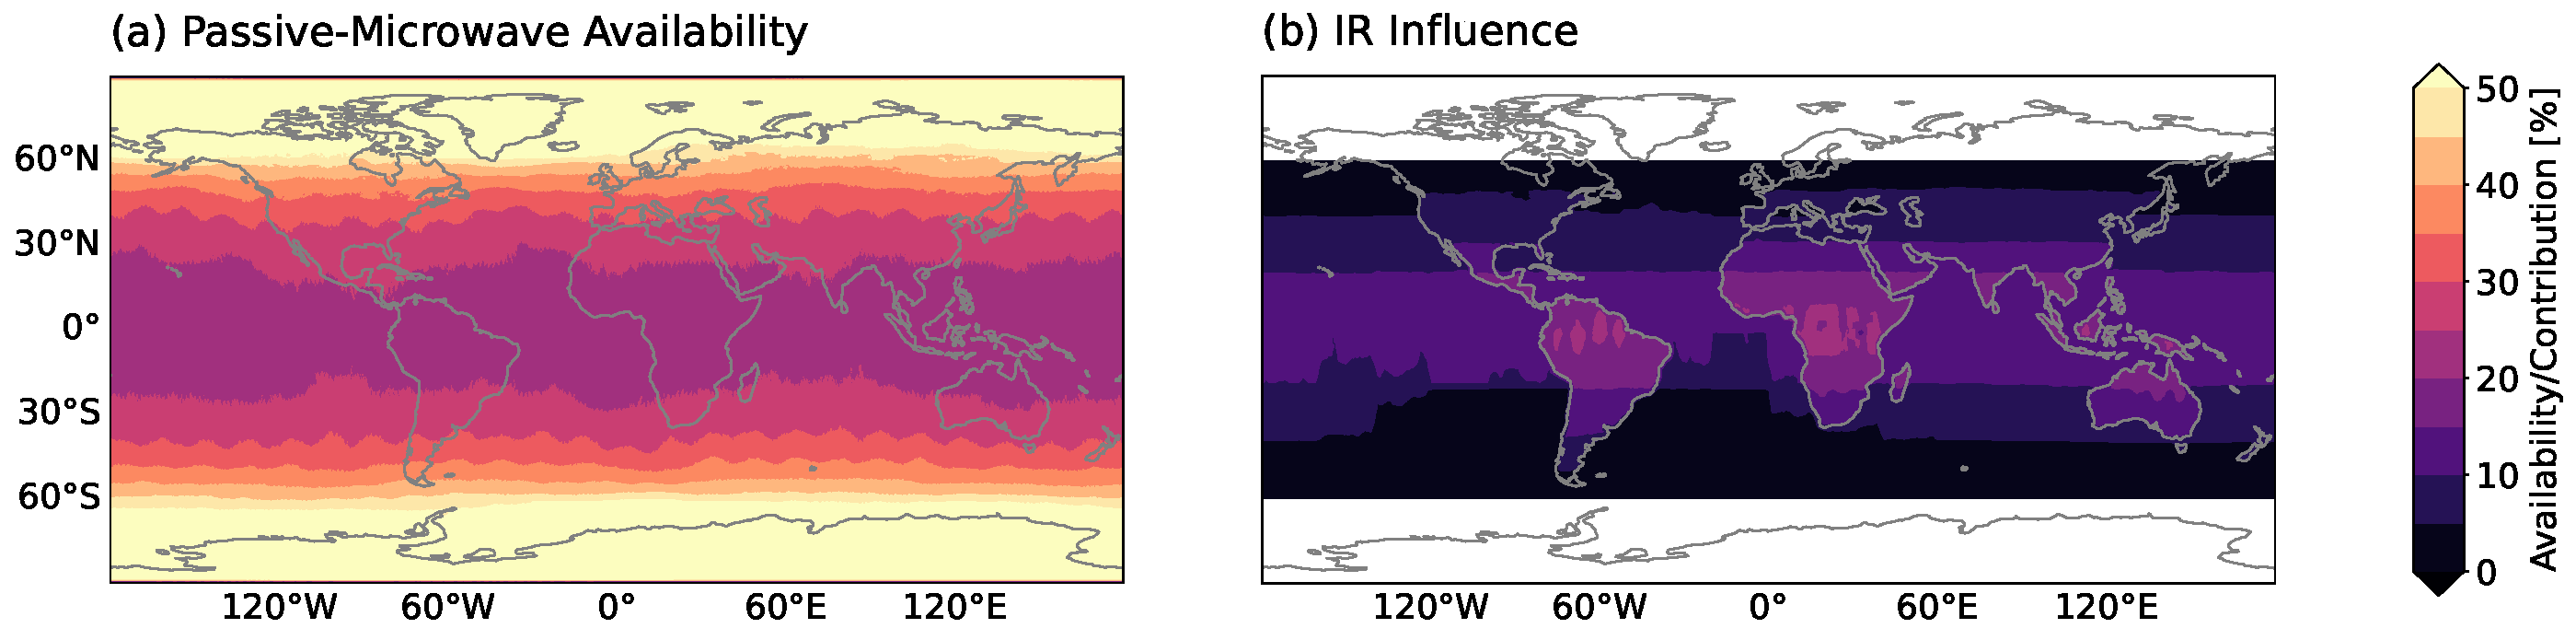
\includegraphics[width=37pc]{figures/figure01.pdf}}
 \caption{
Average availability at any one half-hour of passive microwave observations from 2022-01-01 to 2023-01-01 (a) and relative contribution of infrared (IR) observations (b) to IMERG V07 Final Run merged precipitation estimates.
 }\label{fig:availability}
\end{figure}

This dependence on advected PMW estimates can produce physically implausible
representations of rapidly evolving precipitation systems.
Figure~\ref{fig:evolution} highlights this issue for a convective storm case.
While the precipitation field changes markedly between the first and fourth
half-hourly timesteps, it remains nearly static in the intervening period.
Inspection of the corresponding PMW and IR retrievals shows that this stagnation
coincides with a PMW overpass at 15:00 UTC. In IMERG, PMW estimates are given
exclusive weight within a ±30-minute window around such overpasses
\citep{huffman2019imerg_v07_atbd}, such that any variability during this
interval arises solely from advection of the PMW-derived precipitation rates.
Outside this enforced PMW-only window, IR-based estimates begin to contribute to
the merged field. Because the IR and coincident PMW retrievals differ
substantially, their combination introduces abrupt temporal changes. For this
exmple, the temporal evolution of the merged precipitation is driven more by
inconsistencies between the PMW and IR retrievals than by the underlying
precipitation dynamics.

\begin{figure}[h]
 \centerline{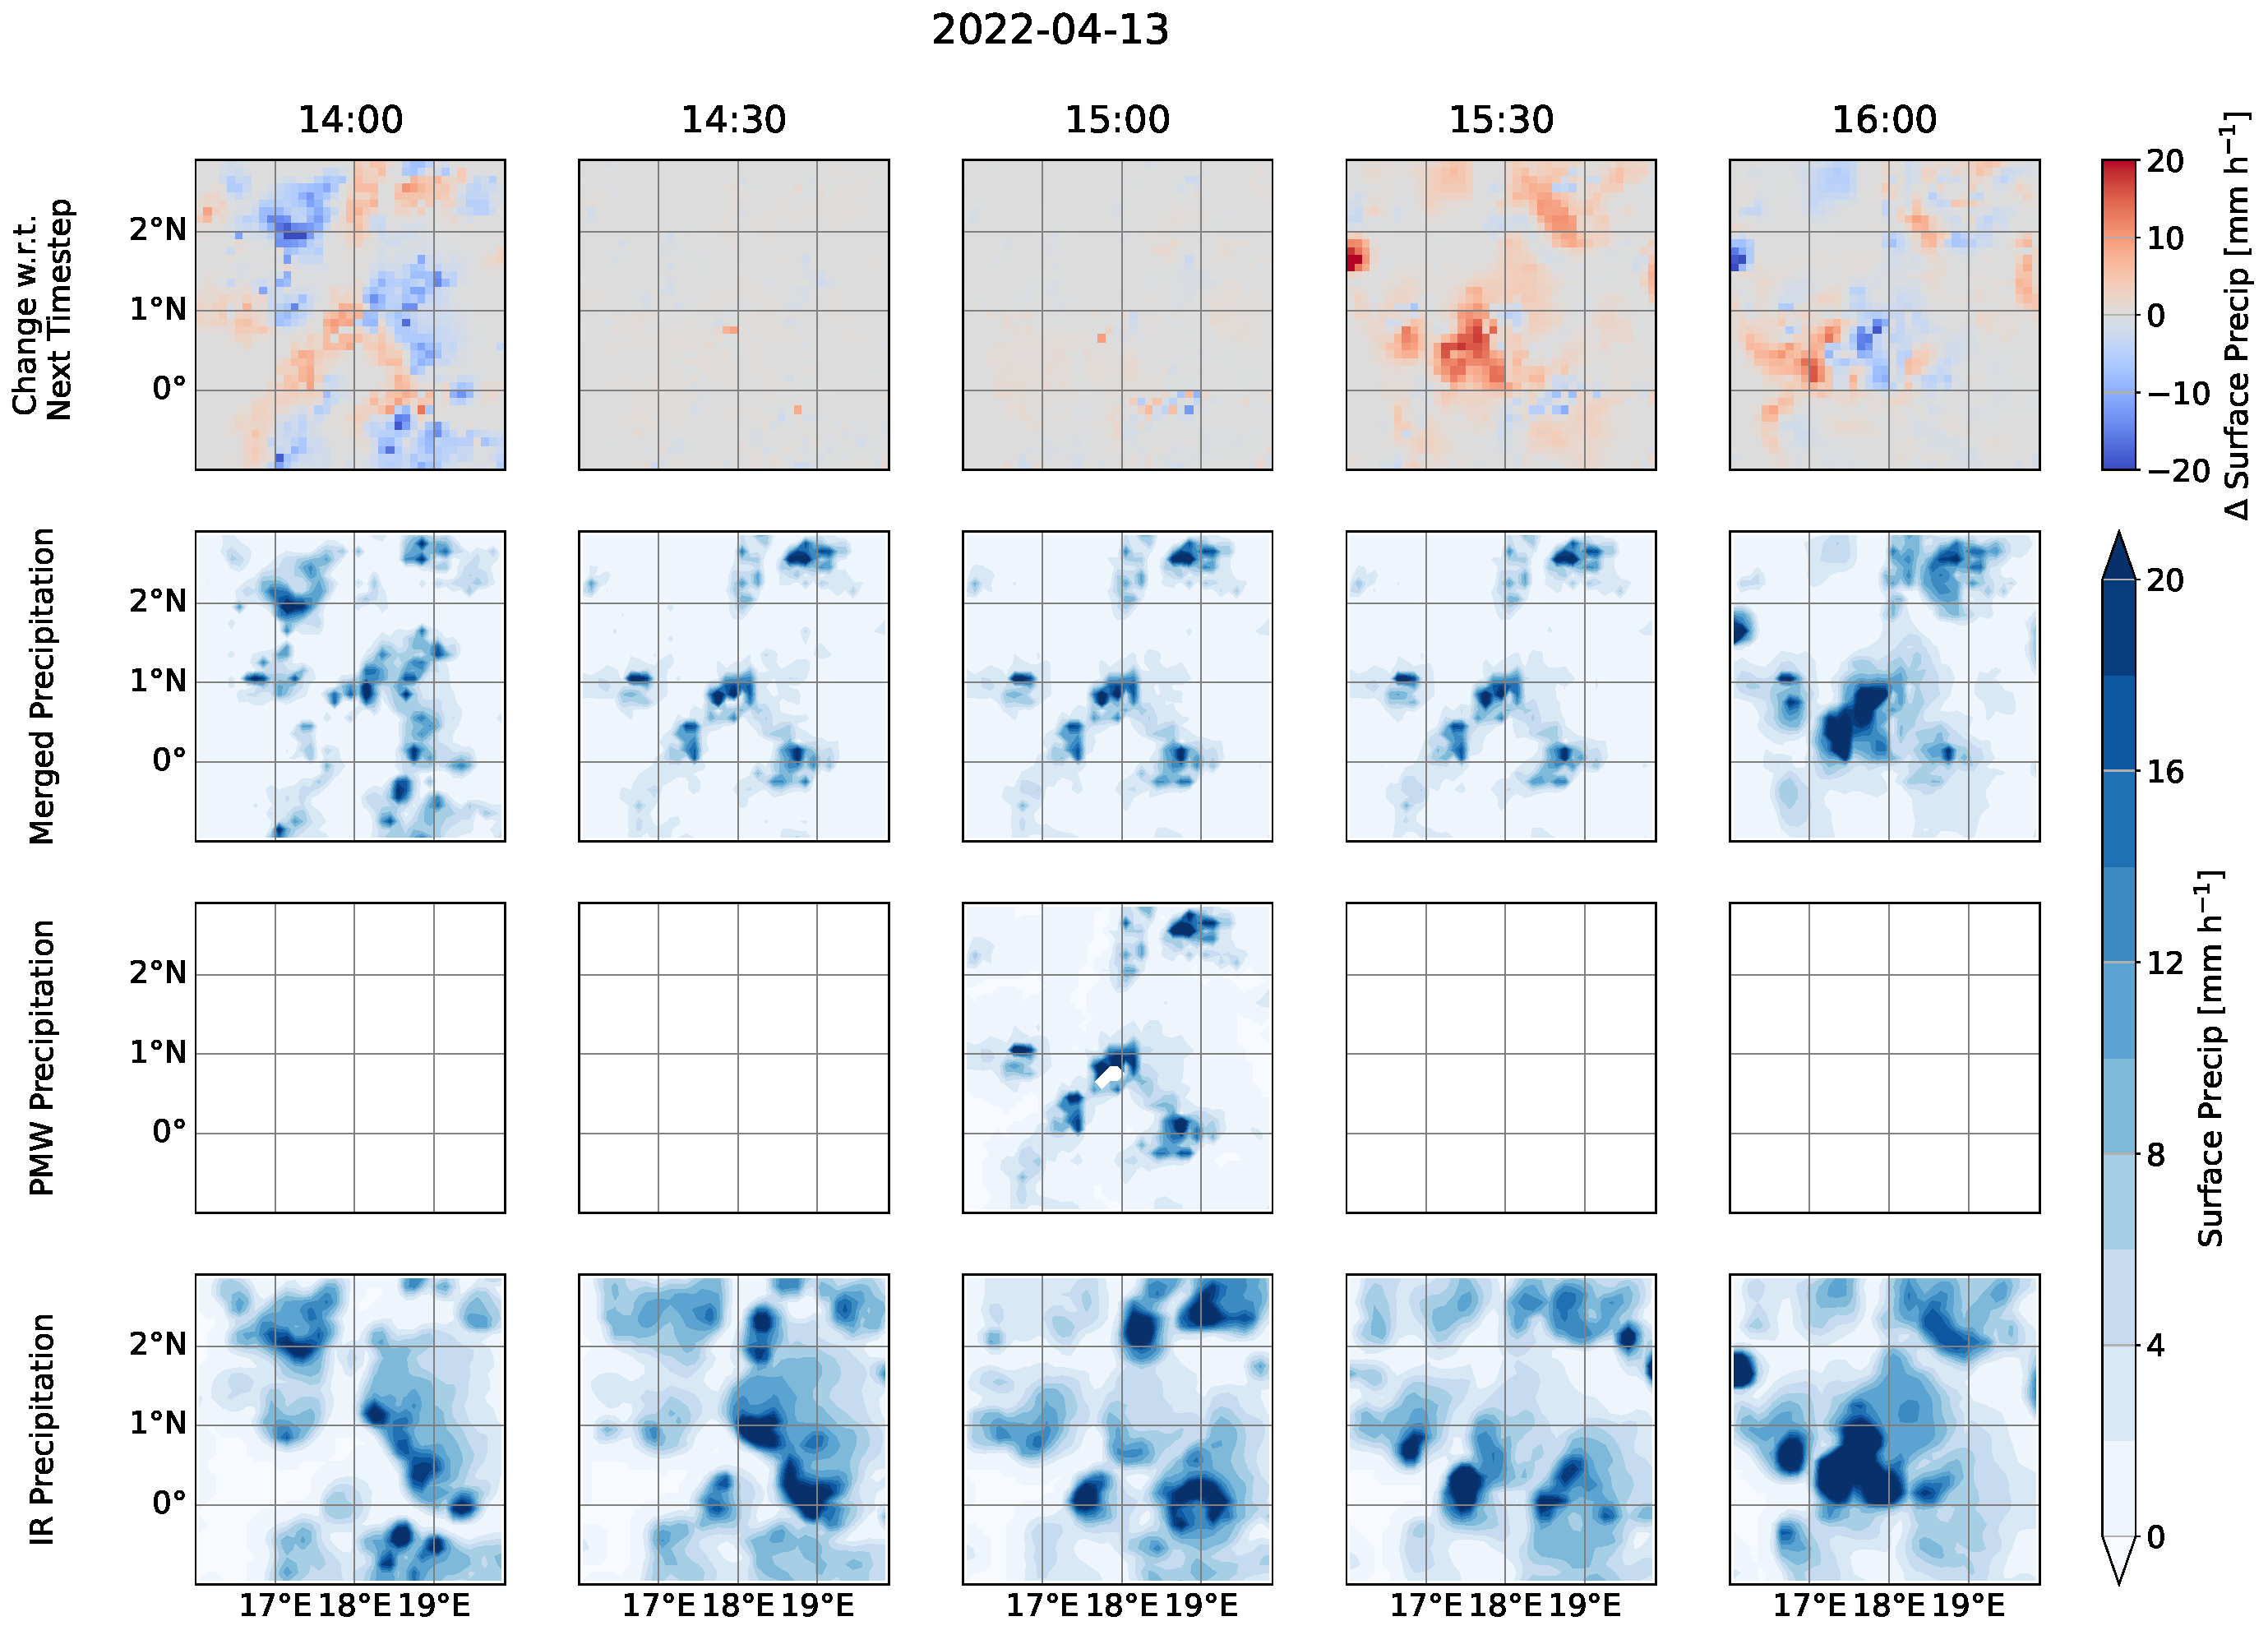
\includegraphics[width=37pc]{figures/figure02.pdf}}
 \caption{
    Evolution of convective precipitation cells in IMERG V07. The five
    columns show the half-hourly precipitation field from 14:00 to
    16:00 UTC on April 13, 2022. The first row shows the change in the precipitation
    field relative to the next time step. Rows 2-4 show the final merged IMERG V07
    precipitation field, the passive-microwave-derived precipitation field, and the
    infrared-derived precipitation field, respectively.
 }\label{fig:evolution}
\end{figure}

The example above underscores the need for more accurate IR-based precipitation
estimates to improve the representation of precipitation processes in merged
products.

Recent work has shown that machine-learning-based retrievals exploiting the
spatial structure of satellite imagery can substantially enhance precipitation
estimates from geostationary observations \citep{amell_probabilistic_2025} ---
even when limited to single-channel IR window measurements
\citep{pfreundschuh_improved_2022}. Building on these advances, this study
introduces the Goddard Profiling Algorithm Infrared (GPROF-IR), a new retrieval
designed to provide improved IR-based background precipitation estimates for
next-generation merged precipitation products. The name GPROF-IR reflects its
intended role as a complement to the GPROF-NN algorithm
\citep{pfreundschuh_gprof-nn_2022}, which will be used to produce PMW
precipitation estimates for IMERG V08; it does not imply that the algorithm
retrieves vertical hydrometeor profiles. GPROF-IR uses a similar convolutional
network model as GPROF-NN to leverage spatial informaiton content in the IR
observaitons. Expanding this approach, GPROF-IR  integrates up to five consecutive
half-hourly IR images into the input. The inclusion of temporal information provides robust accuracy
improvements over the single-time-step baselines demonstrating that the retrieval is
able to leverage information on the evolution of cloud systems to constrain
surface precipitation estimates.



\section{Methods and Data}
\label{sec:methods}

\subsection{Input and Target Data}

\subsubsection{CPC 4-km Gridded IR}

The input data used by the GPROF-IR retrieval are geostationary IR observations
from the NOAA Climate Prediction Center globally merged IR product version 1
\citep{ncep_cpc_gpm_mergir_v1, janowiak2001real}. The CPC IR dataset compiles
geostationary IR observations from the 11-$\mu$m IR window channel from the
global constellation of geostationary satellites on a regular latitude-longitude
grid. The gridded observations at half-hourly resolution cover much
of the globe between $60^\circ$S and $60^\circ$N from 1998 until the present.

\subsubsection{GPM 2BCMB}

We evaluate two sources of target surface precipitation rates used for training
the GPROF-IR retrieval. The first source is derived from the level-2
combined radar–radiometer product (2BCMB \citep{cmb_data}) of the Global Precipitation
Measurement (GPM, \citep{hou_global_2014}). The 2BCMB product
integrates observations from the GPM Dual-Frequency Precipitation Radar (DPR)
and the GPM Microwave Imager (GMI) within a variational retrieval framework,
yielding more accurate precipitation estimates than either sensor alone. It
serves as the primary reference dataset for training PMW retrievals across the
GPM constellation and is widely understood to provide  the most reliable global
precipitation measurements currently available.

\subsubsection{GPROF V08 GMI}

As second source of reference data, we use the GPROF V08 PMW retrieval
from the GMI sensor. GMI is the flagship passive sensor of the GPM constellation
and is among the sensors providing the finest spatial resolution and broadest
spectral coverage. PMW precipitation estimates from GMI are therefore among the most
reliable from the GPM constellation. In fact, \citet{pfreundschuh_gprof_2024} have shown
that the accuracy of GMI-based precipitation estimates is comparable to that of
2BCMB when compared against gauge-corrected ground-based radar over CONUS.

GPROF V08 -- the next operational version of the Goddard Profiling Algorithm
(GPROF, \citet{kummerow2015evolution}) -- will use an updated version of the
GPROF-NN 3D retrieval presented in \citep{pfreundschuh_gprof-nn_2022}. While the
GPROF V08 retrieval is also based on reference precipitation rates from the GPM
2BCMB product, it implements several ad-hoc solutions to address shortcomings of
the reference data. Among others, these include the use reference precipitation
estimates from ground-based radar over snow-covered surfaces and the filling-in
of light and frozen oceanic precipitation that is missed by the DPR using the
GPROF-NN XPR retrieval \citep{pfreundschuh_xpr_2026}.

\subsection{Baseline Precipitation Estimates}

Since the purpose of GPROF-IR is to provide improved precipitation estimates for
the upcoming version of the IMERG, we compare the GPROF-IR precipitation rates
against PMW and IR precipitation estimates from the current IMERG V07 product.
Specifically, we use precipitation estimates from the IMERG Final run
\citep{gpm_imerg_final_v07}. IMERG V07 uses a Kalman-filter-based merging scheme
\citep{huffman2019imerg_v07_atbd} to combine PMW precipitation rates from GPROF
V07 and the Persiann dynamic infrared--rain rate (PDIR-now) retrieval
\citep{nguyen2020persiann}. Where possible we will consider the accuracy of the
PMW and IR-based estimates separately using the \textit{MWPrecipitation} and
\textit{IRPrecipitation} fields from IMERG V07.

As an additional baseline, we use precipitation estimates from the ERA5
reanalysis dataset \citep{hersbach_era5_2020}. ERA5 is the leading global
reanalysis dataset providing continuous global coverage at hourly temporal
resolution and a spatial resolution of 0.25$^\circ$. ERA5 provides global
precipitation estimates since 1940 and therefore constitutes an alternative to
global merged satellite precipitation products for studying the evolution of precipitation
systems. In contrast to satellite-based precipitation products, which generally
estimate precipitation rates directly from observations, ERA5 uses a numerical
weather prediction model to determine the atmospheric state that provides the
best agreement with a wide range of meteorological observations.

Finally, we also compare global precipitation distributions from the GPROF-IR
retrievals to the GPCP V3.3 \citep{gpcp_v33_precip} precipitation climatology.
GPCP combines satellite and gauge precipitation measurements to provide a
high-quality precipitation record for climate applications. Since GPCP is
generally considered the best global precipitation record for climate
applications, it provides an important reference point for the GPROF-IR
retrievals.

\subsection{Validation Data}

To demonstrate the improved skill of the GPROF-IR retrieval compared to IMERG
V07 and ERA5 baselines, we evaluate the retrievals using multiple sources of
independent validation data.

\subsubsection{The SatRain Benchmark Dataset}

The SatRain benchmark dataset \citep{pfreundschuh2026benchmark} provides a
machine-learning-ready training and evaluation dataset for machine-learning
precipitation retrievals. It integrates high-quality reference data from
gauge-corrected ground radars and the WegenerNet high-density gauge network
\citep{fuchsberger_wegenernet_2021}. The testing split of the benchmark provides
an easily accessible and comprehensive validation resource to for satellite
precipitation retrievals. By using the publicly available SatRain dataset
and following its standardized evaluation protocol, we ensure that the
validation results of the GPROF-IR retrievals are reproducible and directly
comparable to other algorithms.

The analysis presented here uses the GMI-based testing data, which comprises one
year of GMI overpasses over CONUS and Korea as well as two years of overpasses
over the Wegener gauge network in Austria. The CONUS testing data is derived
from gauge-corrected precipitation estimates from the NOAA Multi-Radar
Multi-Sensor (MRMS, \citep{smith_multi-radar_2016}) products; the Korea data is
derived from gauge-corrected precipitation estimates provided by the Korean
Meteorological Agency \citep{ryu_radar_2025}. To accommodate for the testing
resolution of 0.036 degree used by the SatRain dataset, all GPROF-IR results are
interpolated to the SatRain grid using bi-linear interpolation.


\subsubsection{OceanRAIN Shipborne Distrometer Measurements}

Since the SatRain benchmark dataset relies on measurements from gauges and
gauge-corrected ground-based radars, it is limited to land surfaces. To also
validate the retrievals over ocean, we use shipborne distrometer measurements
from the OceanRAIN dataset \citep{klepp2018oceanrain} from all measurements
available during the years 2017 and 2019. The SatRain measurement are provided
at 1-min temporal resolution, which we average over 30 min centered on the
nominal time of corresponding GPROF-IR retrieval. The spatial distribution of
the OceanRAIN--GPROF-IR match-ups are shown in Fig.~\ref{fig:ocean_rain}. Since
the validation period overlaps with the training data, we exclude all
measurements that coincide with GMI overpasses, which were used to create the
training data for GPROF-IR. This excludes any observations that the retrieval
may have encountered during training and should therefore avoid potential
positive biases in the validation due to data leakage.

\begin{figure}[h]
 \centerline{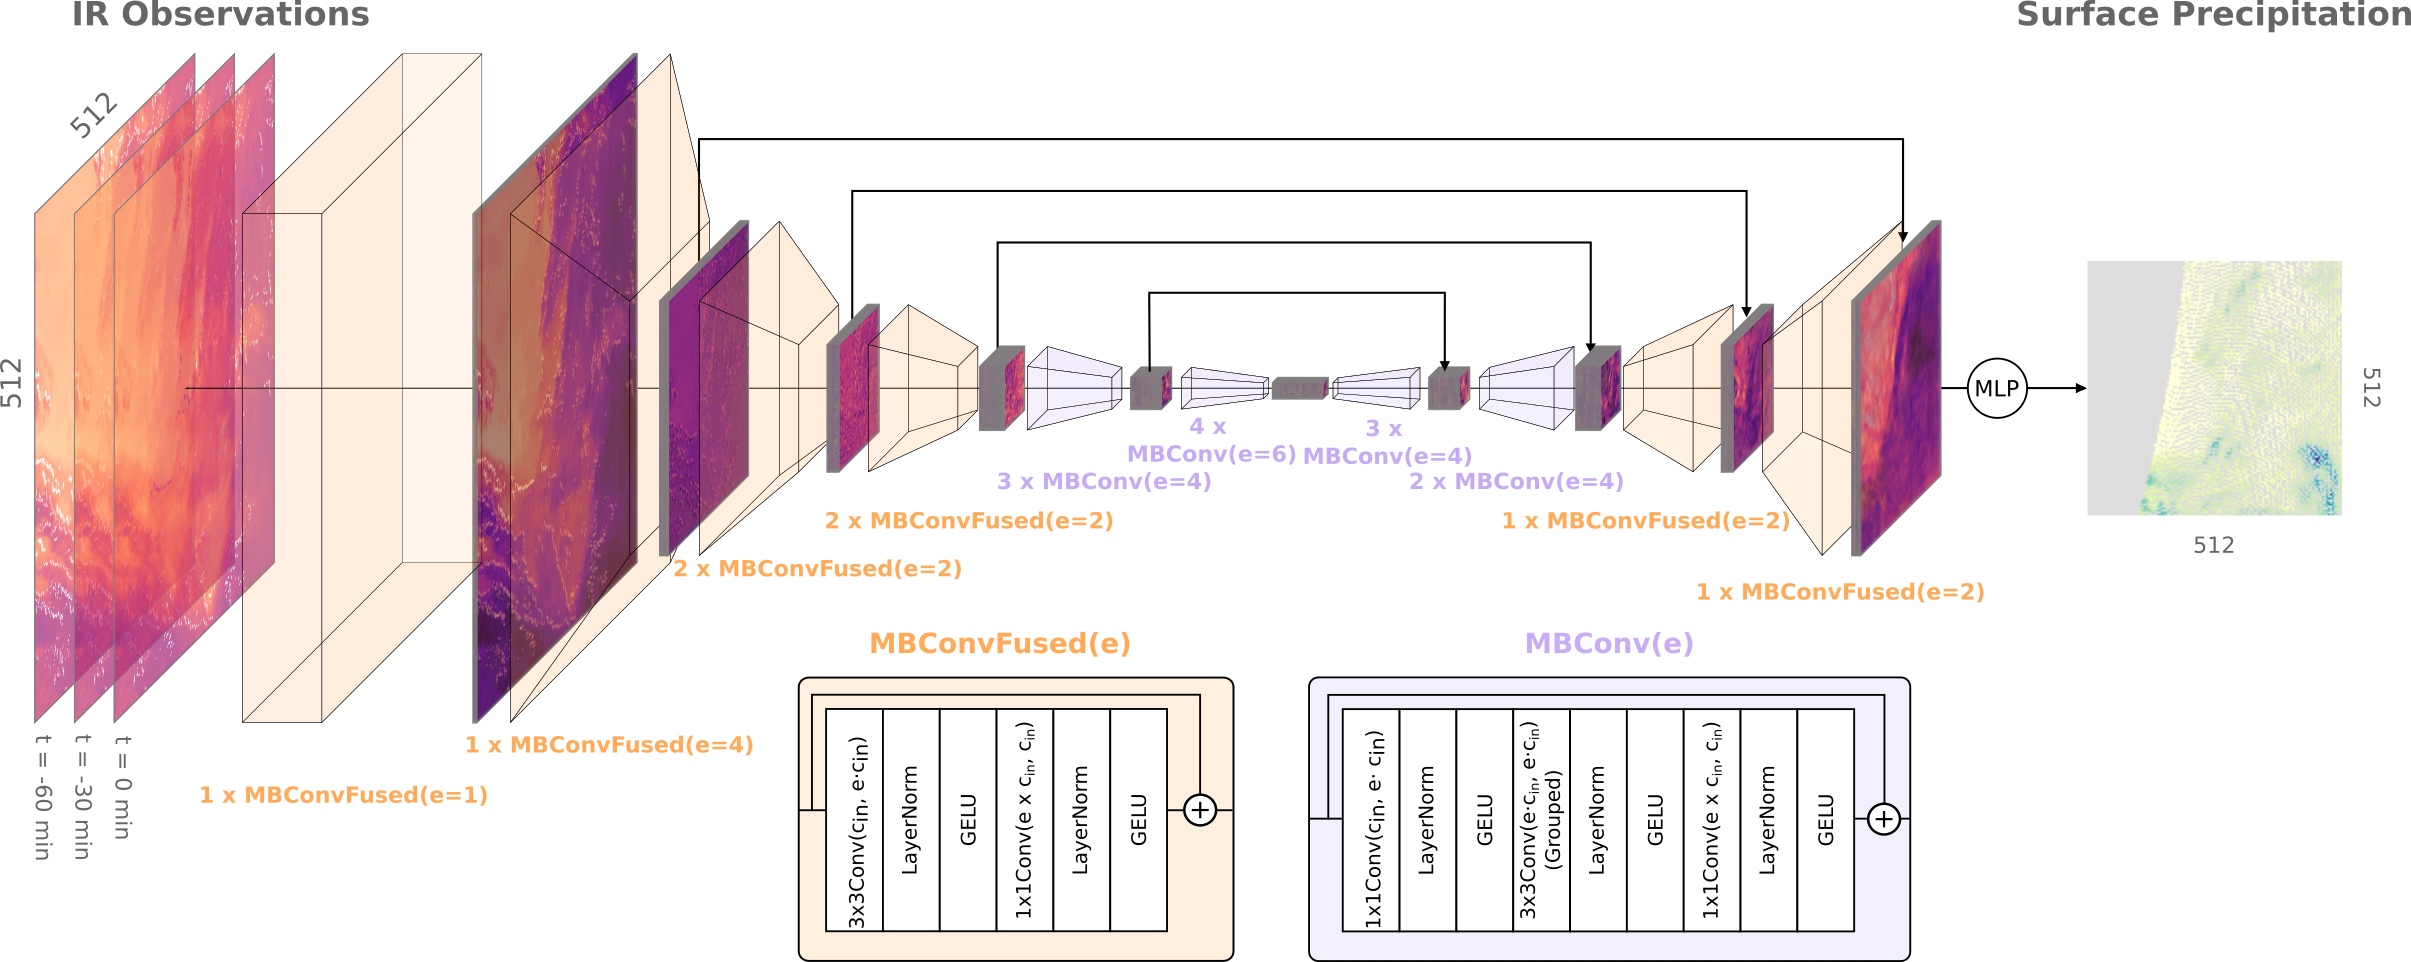
\includegraphics[width=37pc]{figures/figure03.png}}
 \caption{
   Zonal (a) and global (b) counts of matched OceanRAIN shipborne distrometer
   estimates and corresponding satellite precipitation estimates used to
   validate the GPROF-IR retrieval.
 }\label{fig:ocean_rain}
\end{figure}


\subsection{Implementation}
\subsubsection{Neural Network Model}

The GPROF-IR retrieval is based on the same U-Net \citep{ronneberger_u-net_2015} architecture used for the
GPROF V08 retrieval. The network – as illustrated in Fig. 2 – is composed of
EfficientNet-V2–style inverted bottleneck convolutional blocks \citep{tan_efficientnetv2_2021}.
Following the normalization and activation design adopted in ConvNeXt \citep{liu_convnet_2022}, each convolutional block uses Layer Normalization \citep{ba2016layer}
and GELU activation functions \citep{hendrycks2016gaussian}. Compared to the
architecture of the GPROF V08 models, both width and depth of the model were
reduced in order to accommodate operational requirements on processing time.
Note that \textit{model} is used in this paper to denote a neural network model, not to
be confused with a numerical model of precipitation, weather, or climate
processes.

The retrieval input consists of single-channel infrared observations from up to
five consecutive timesteps leading up to the nominal time. Preceding timesteps
were used instead of centered timesteps to avoid impacting the latency of
near-real-time retrievals. \\

To leverage the comparably high resolution of the IR input observations, the
model ingests the gridded IR observations at their native 0.036$^\circ$ and 30
min resolution. Since the effective spatial resolution of the retrieved
precipitation can be expected to be much lower than the 0.036$^\circ$ of the
input observations, the model output is produced at half of the input spatial
resolution to reduce inference complexity as well as storage requirements. The
input consists of image patches of size 512 px x 512 px at 0.036$^\circ$-resolution
that are mapped to precipitation estimates of size 256 px $\times$ 256 px with a
resolution of 0.072$^\circ$. The model outputs are therefore at a spatial
resolution of 0.072$^\circ$ and a temporal resolution of 30 minutes.

The training dataset comprises IR observations paired with corresponding
reference precipitation estimates within $\pm$15 minutes of the nominal
observation time. The model is trained using all available reference data from
2015–2018, while independent data from 2022 are used for evaluation of retrieval
performance. The network is trained to predict 32 quantiles of the posterior
distribution of the target precipitation rate using a quantile-regression loss
\citep{pfreundschuh_neural_2018}. The principal retrieval output is the mean of
the posterior distribution calculated from these 32 quantiles by approximating
the cumulative distribution function and calculating its mean. The resulting
posterior mean is approximately bias free and minimizes the mean-squared error
of retrieval output. However, the probabilistic nature of the network also
allows the calculation of other statistical properties of the posterior
distribution such as exceedance probability for arbitrary precipitation rates,
which we will use later to assess the precipitation detection capabilities of
the model. All retrievals have been trained for 140 epochs using the AdamW
optimizer \citep{loshchilov_decoupled_2019} lwith a learning rate of
$5 \cdot 10^{4}$, a cosine-annealing learning rate schedule, and warm restarts
\citep{loshchilov2016sgdr} after 20 and 60 epochs.


\begin{figure}[h]
 \centerline{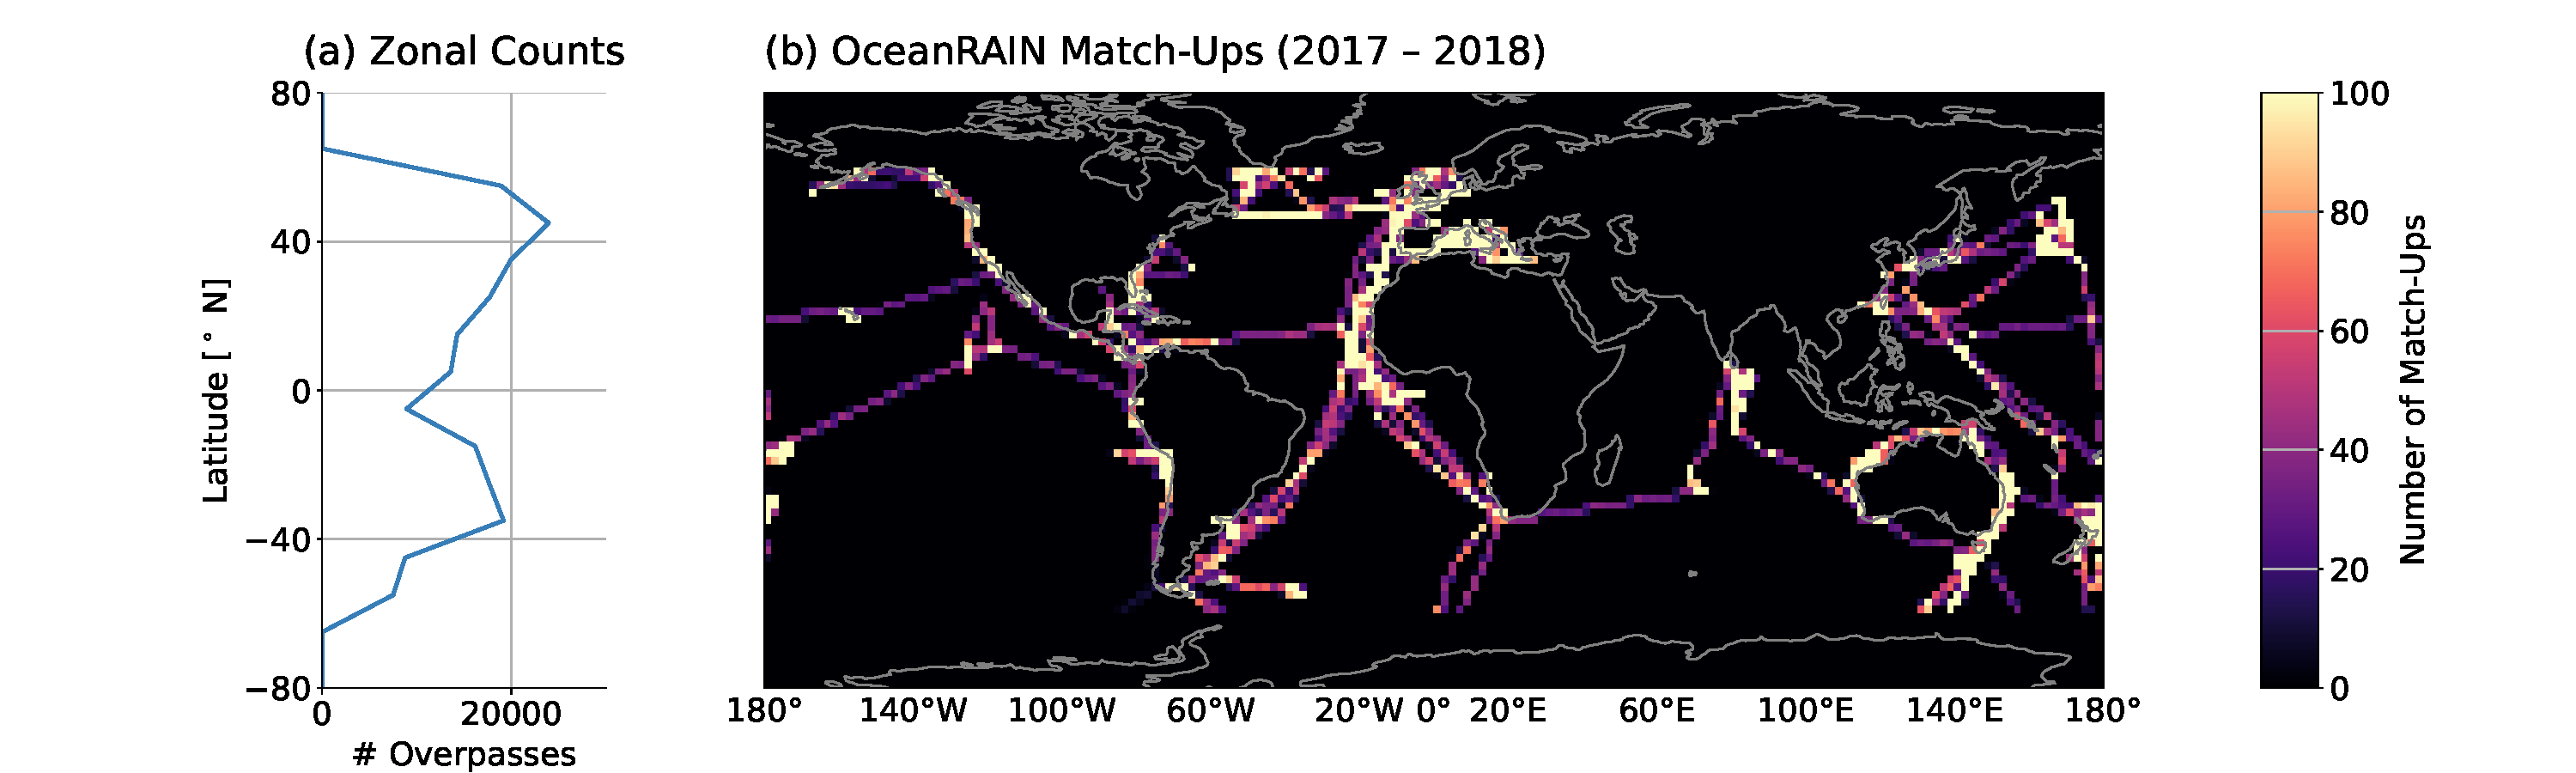
\includegraphics[width=37pc]{figures/figure03.pdf}}
 \caption{
The neural network architecture used to implement the GPROF-IR retrieval.
 }\label{fig:achictecture}
\end{figure}

\subsubsection{Design Experiments}

Gridded geostationary IR observations provide only indirect information on
surface precipitation, as they are primarily sensitive to cloud-top properties.
However, their high temporal resolution captures the evolution of cloud systems,
which can help constrain precipitation at the surface. To exploit this temporal
information, we evaluate retrieval configurations that incorporate multiple
preceding IR timesteps. Specifically, we consider models that include two and
four additional prior observations (for a total of three and five timesteps,
respectively). These multi-timestep models are trained sequentially: the
single-timestep model is trained first, its weights are used to initialize the
three-timestep model, and the latter is subsequently used to initialize the
five-timestep model.

Overall, we test the following retrieval configurations:

\begin{description}
    \item[GPROF-IR (CMB, 1)] uses input observations from a single time step and
      is trained using the 2BCMB dataset as reference data.
    \item[GPROF-IR (GMI, 1)] uses input observations from a single time step and
      trained using GPROF V08 GMI retrieval results as reference data.
    \item[GPROF-IR (GMI, 3)] uses input observations from three time steps and
      trained using GPROF V08 GMI retrieval results as reference data.
    \item[GPROF-IR (GMI, 5)] uses input observations from five time steps and
      trained using GPROF V08 GMI retrieval results as reference data.
\end{description}

\section{Results}
\label{sec:results}

Below we asses the retrieval accuracy of GPROF-IR, validate it using
independent precipitation estimates, and characterize the resulting global
precipitation climatology.

\subsection{Test-Set Accuracy}

\begin{figure}[h]
 \centerline{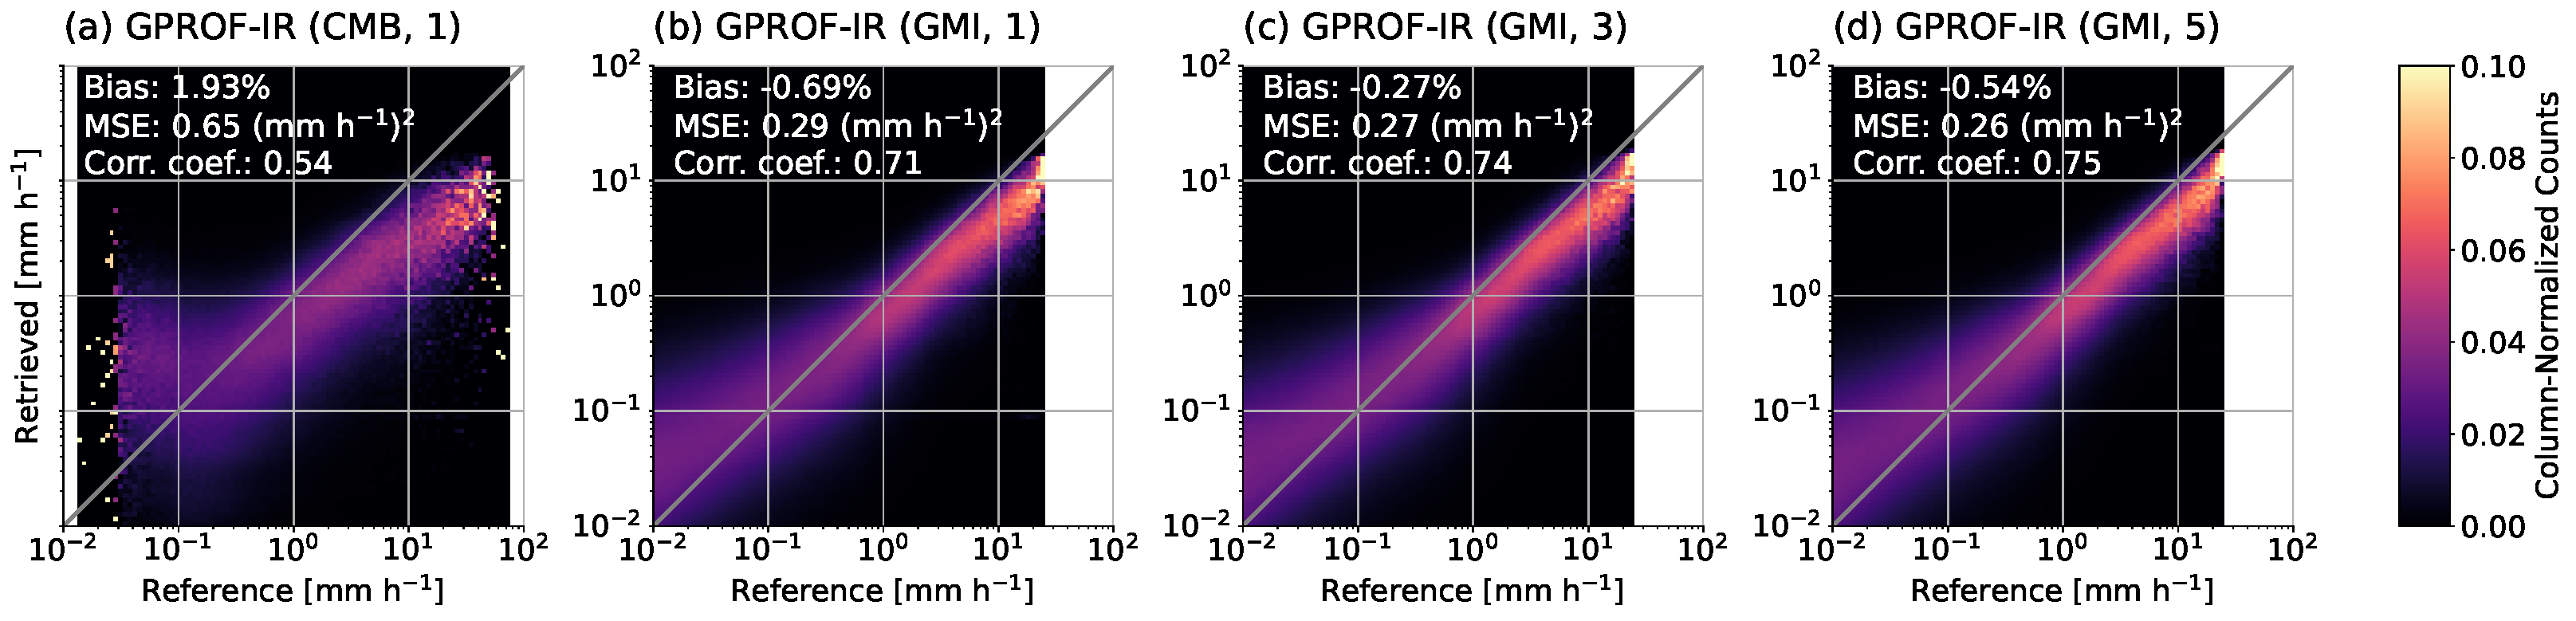
\includegraphics[width=37pc]{figures/figure05.pdf}}
 \caption{
Test-set accuracy of the GPROF-IR retrieval. Each panel shows a scatter plot
showing the relation between reference and retrieved precipitation for (a) the
single-step retrieval using GPM 2BCMB reference data, (b) the single-step
retrieval using GPROF-NN GMI reference data, (c ) a three-step retrieval using
GMI reference data, and (d) a 5-step retrieval using GMI reference data.
 }\label{fig:test_results}
\end{figure}

We begin by assessing the retrieval accuracy on temporally independent testing
data from the year 2022. Similar to the training data, the testing data for the
different GPROF-IR configurations uses different target precipitation estimates.
The testing data for the GPROF-IR (CMB, 1) configuration uses reference estimates
from 2BCMB whereas the other configurations use estimates from GPROF V08 GMI.

Figure 3 displays scatter plots and accuracy statistics for the four tested
retrieval configurations. All four retrievals demonstrate skill in reproducing
the reference precipitation estimates with low biases and mean-squared error and
high correlation coefficients. However, they also exhibit a tendency to
overestimate light precipitation and underestimate heavy precipitation, which
is typically observed for precipitation retrievals from passive sensors. The GPROF-IR (CMB, 1)
retrieval exhibits notably larger spread than the GPROF V08 GMI-based
retrievals, which is a result of the higher spatial resolution of the 2BCMB
reference data. The three-timestep retrieval GPROF-IR (GMI, 3) shows small but
notable improvements over the single-timestep GMI retrieval indicating that it
is able to leverage temporal information in the IR imagery to better constrain
precipitation estimates. The GPROF-IR (GMI, 5) retrieval shows further, but
smaller improvements over the three-step retrieval, indicating that the
information extractable from the temporal evolution may begin to plateau.

\subsection{Validation}

To provide a fair assessment of the GPROF-IR retrievals, we compare them
to baseline precipitation estimates from IMERG V07 and ERA5 using independent
precipitation estimates from the SatRain testing dataset and shipborne
distrometer measurements from the OceanRAIN dataset as reference data.

\subsubsection{SatRain}

Figure~\ref{fig:results_satrain} shows the evaluation metrics of the GPROF-IR
retrievals and the IMERG and ERA5 baselines assessed across the three testing
domains of the SatRain dataset. In terms of biases, all baselines and models
exhibit similar tendencies: Strong positive biases over the Austria domain, weak
positive to no biases over CONUS, and moderate negative biases over Korea. The
regional differences in the biases are larger than the differences between the
different datasets. This indicates that they are mostly driven by either the
limited capability of remotely sensed and reanalysis precipitation estimates to
capture regional precipitation variability or inconsistencies in the reference
estimates.

In terms of mean absolute error, mean squared error, and correlation
coefficient, the GMI-based GPROF-IR (GMI, 1) retrieval performs consistently as
good or better than the 2BCMB-based GPROF-IR (CMB, 1) retrieval, indicating that
either the increased training data size or the improved representation of light
precipitation and precipitation over snow-covered surfaces of the GPROF V08
reference data increases the retrieval accuracy. In terms of the
incorporation of temporal information, the validation results confirm the
findings from the testing data: While the use of three timesteps yields a robust
improvement in retrieval accuracy, ingesting five instead of three timesteps
yields only marginal benefits.

The GPROF-IR retrieval greatly improves MAE, MSE, and linear correlation
compared to the IMERG V07 IR precipitation estimates. Over the Austria and CONUS
domains, the GPROF-IR algorithms achieve better MSE and correlation coefficient
than IMERG PMW precipitation estimates. Since the evaluation uses SatRain
testing data from GMI overpasses, the IMERG PMW estimates are derived from GMI
observations, which is among the most capable sensors of the GPM constellation.
The GPROF-IR retrievals are thus on par with the best-case accuracy of IMERG V07
over these domains. It should be noted that the PMW retrievals in IMERG V07 use
the Bayesian approach instead of the novel GPROF-NN framework, which will be
used in IMERG V08. For the Korea domain, the GPROF-IR accuracy stays below that
of the IMERG PMW estimates. This is likely because the data from the Korea
domain contains relatively more precipitation estimates over water surfaces,
where most PMW sensors have higher information content. Additionally, warm
precipitation with lower cloud tops and thus weaker signatures in the IR imagery
plays a larger role over the Korea domain than over CONUS, which may further
contribute to the relatively lower accuracy of the IR retrievals
compared to the IMERG GMI estimates.


\begin{figure}[h]
 \centerline{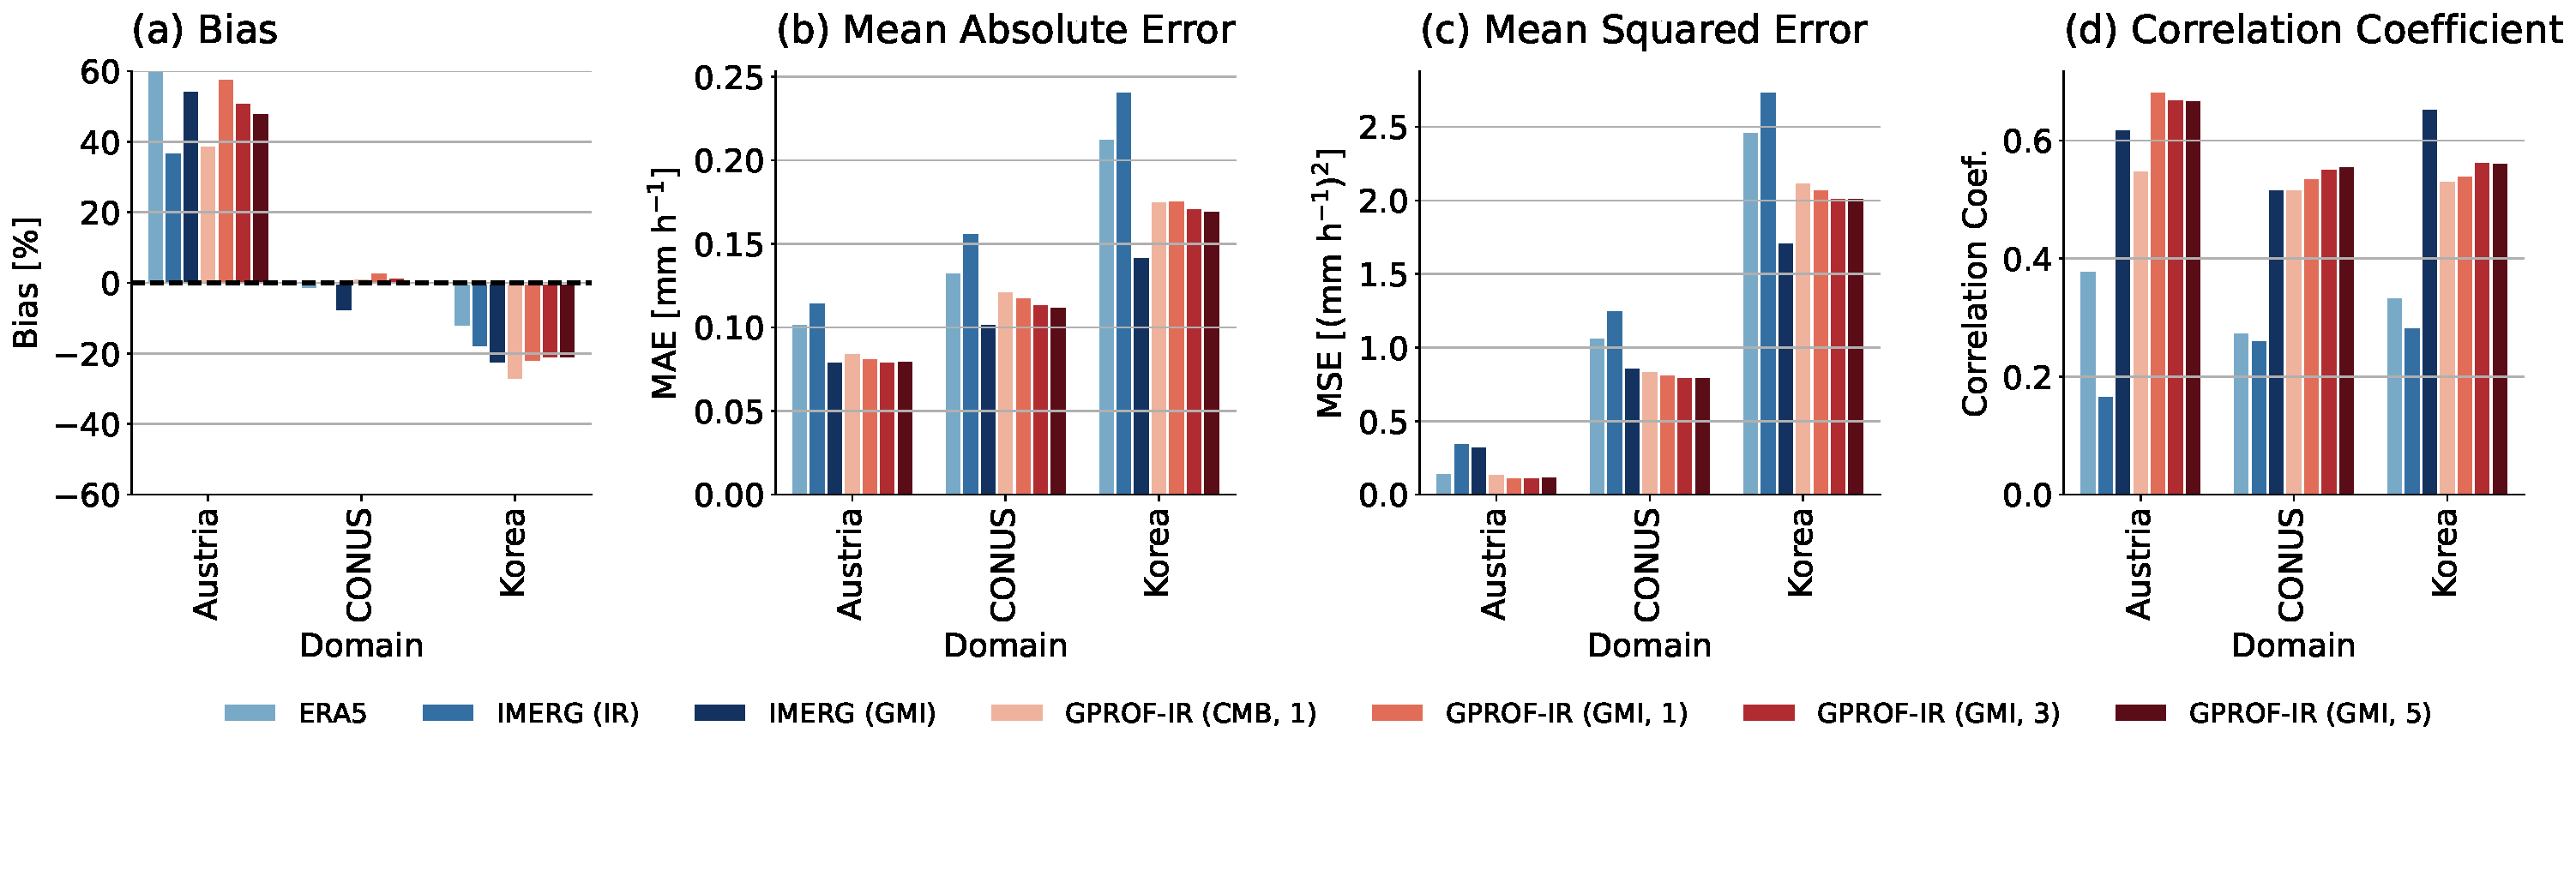
\includegraphics[width=37pc]{figures/figure06.pdf}}
 \caption{
GPROF-IR retrieval accuracy assessed against baseline retrievals using the SatRain benchmark dataset. Panels (a) – (d) compare bias, mean absolute error, mean squared error, and correlation coefficient of the four GPROF-IR configurations against ERA5 and IMERG baselines. Each panel shows results from the CONUS, Korea, and Austria testing domains of the Satrain benchmark dataset.
 }\label{fig:results_satrain}
\end{figure}

\paragraph{Effective Resolution}

 The effective resolution is defined as the smallest spatial scale at which the
spectral coherence exceeds $\sqrt{\frac{1}{2}}$. This corresponds to the
smallest horizontal extent of a precipitation feature for which the
signal-to-noise ratio of the captured spatial variability exceeds one. Since the
analysis of the effective resolution requires spatially continuous precipitation
fields covering at least the resolved scales, the SatRain dataset only allows
assessing the effective resolution over the CONUS and Korea domains.

The spectral coherence curves for the CONUS and Korea domains are shown in
Fig.~\ref{fig:spectral_coherence}. Over CONUS, GPROF-IR (GMI, 5) and GPROF-IR
(GMI, 3) configuration achive effective resolutions of 0.6$^\circ$ whereas the
GPROF-IR (GMI, 1) achieves an effective resolution of 0.63. The 2BCMB-based
retrieval only achieves an effective resolution of 0.9$^\circ$. Over the Korea
domain, the effective resolutions are lower with resolutions around 0.84$^\circ$
for the GPROF-IR (GMI, 3) and 1.07$^\circ$ for the GPROF-IR (GMI, 5) retrieval
whereas and the GPROF-IR (GMI, 1) and GPROF-IR (CMB) configurations do not reach
the $\sqrt{\frac{1}{2}}$ threshold within the resolved scale range.

 The GPROF-IR (GMI, 3) and GPROF-IR (GMI, 5) retrievals achieve effective
resolutions that are about 25\% finer than the GMI-based IMERG V07 PMW estimates
over CONUS. However, the situation is reversed over the Korea domain, where the
IMERG V07 GMI precipitation estimates are about 33 \% finer than the best
GPROF-IR retrievals. Both the IMERG IR and ERA5 precipitation fields stay far
below the $\sqrt{\frac{1}{2}}$ threshold throughout the resolved scale range indicating
that they can't reliably resolve precipitation structures finer than
$1.4^\circ$. These results highlight the substantial improvements in retrieval
accuracy achieve by the GPROF-IR retrieval. GPROF-IR outperforms conventional
PMW retrievals in terms of MSE, linear correlation, and effective resolution
over the assessed continental climate zones and closes much of the gap that
existed between conventional IR and conventional PMW retrievals over sea
surfaces and climates with larger contributions from shallow precipitation.

\begin{figure}[h]
 \centerline{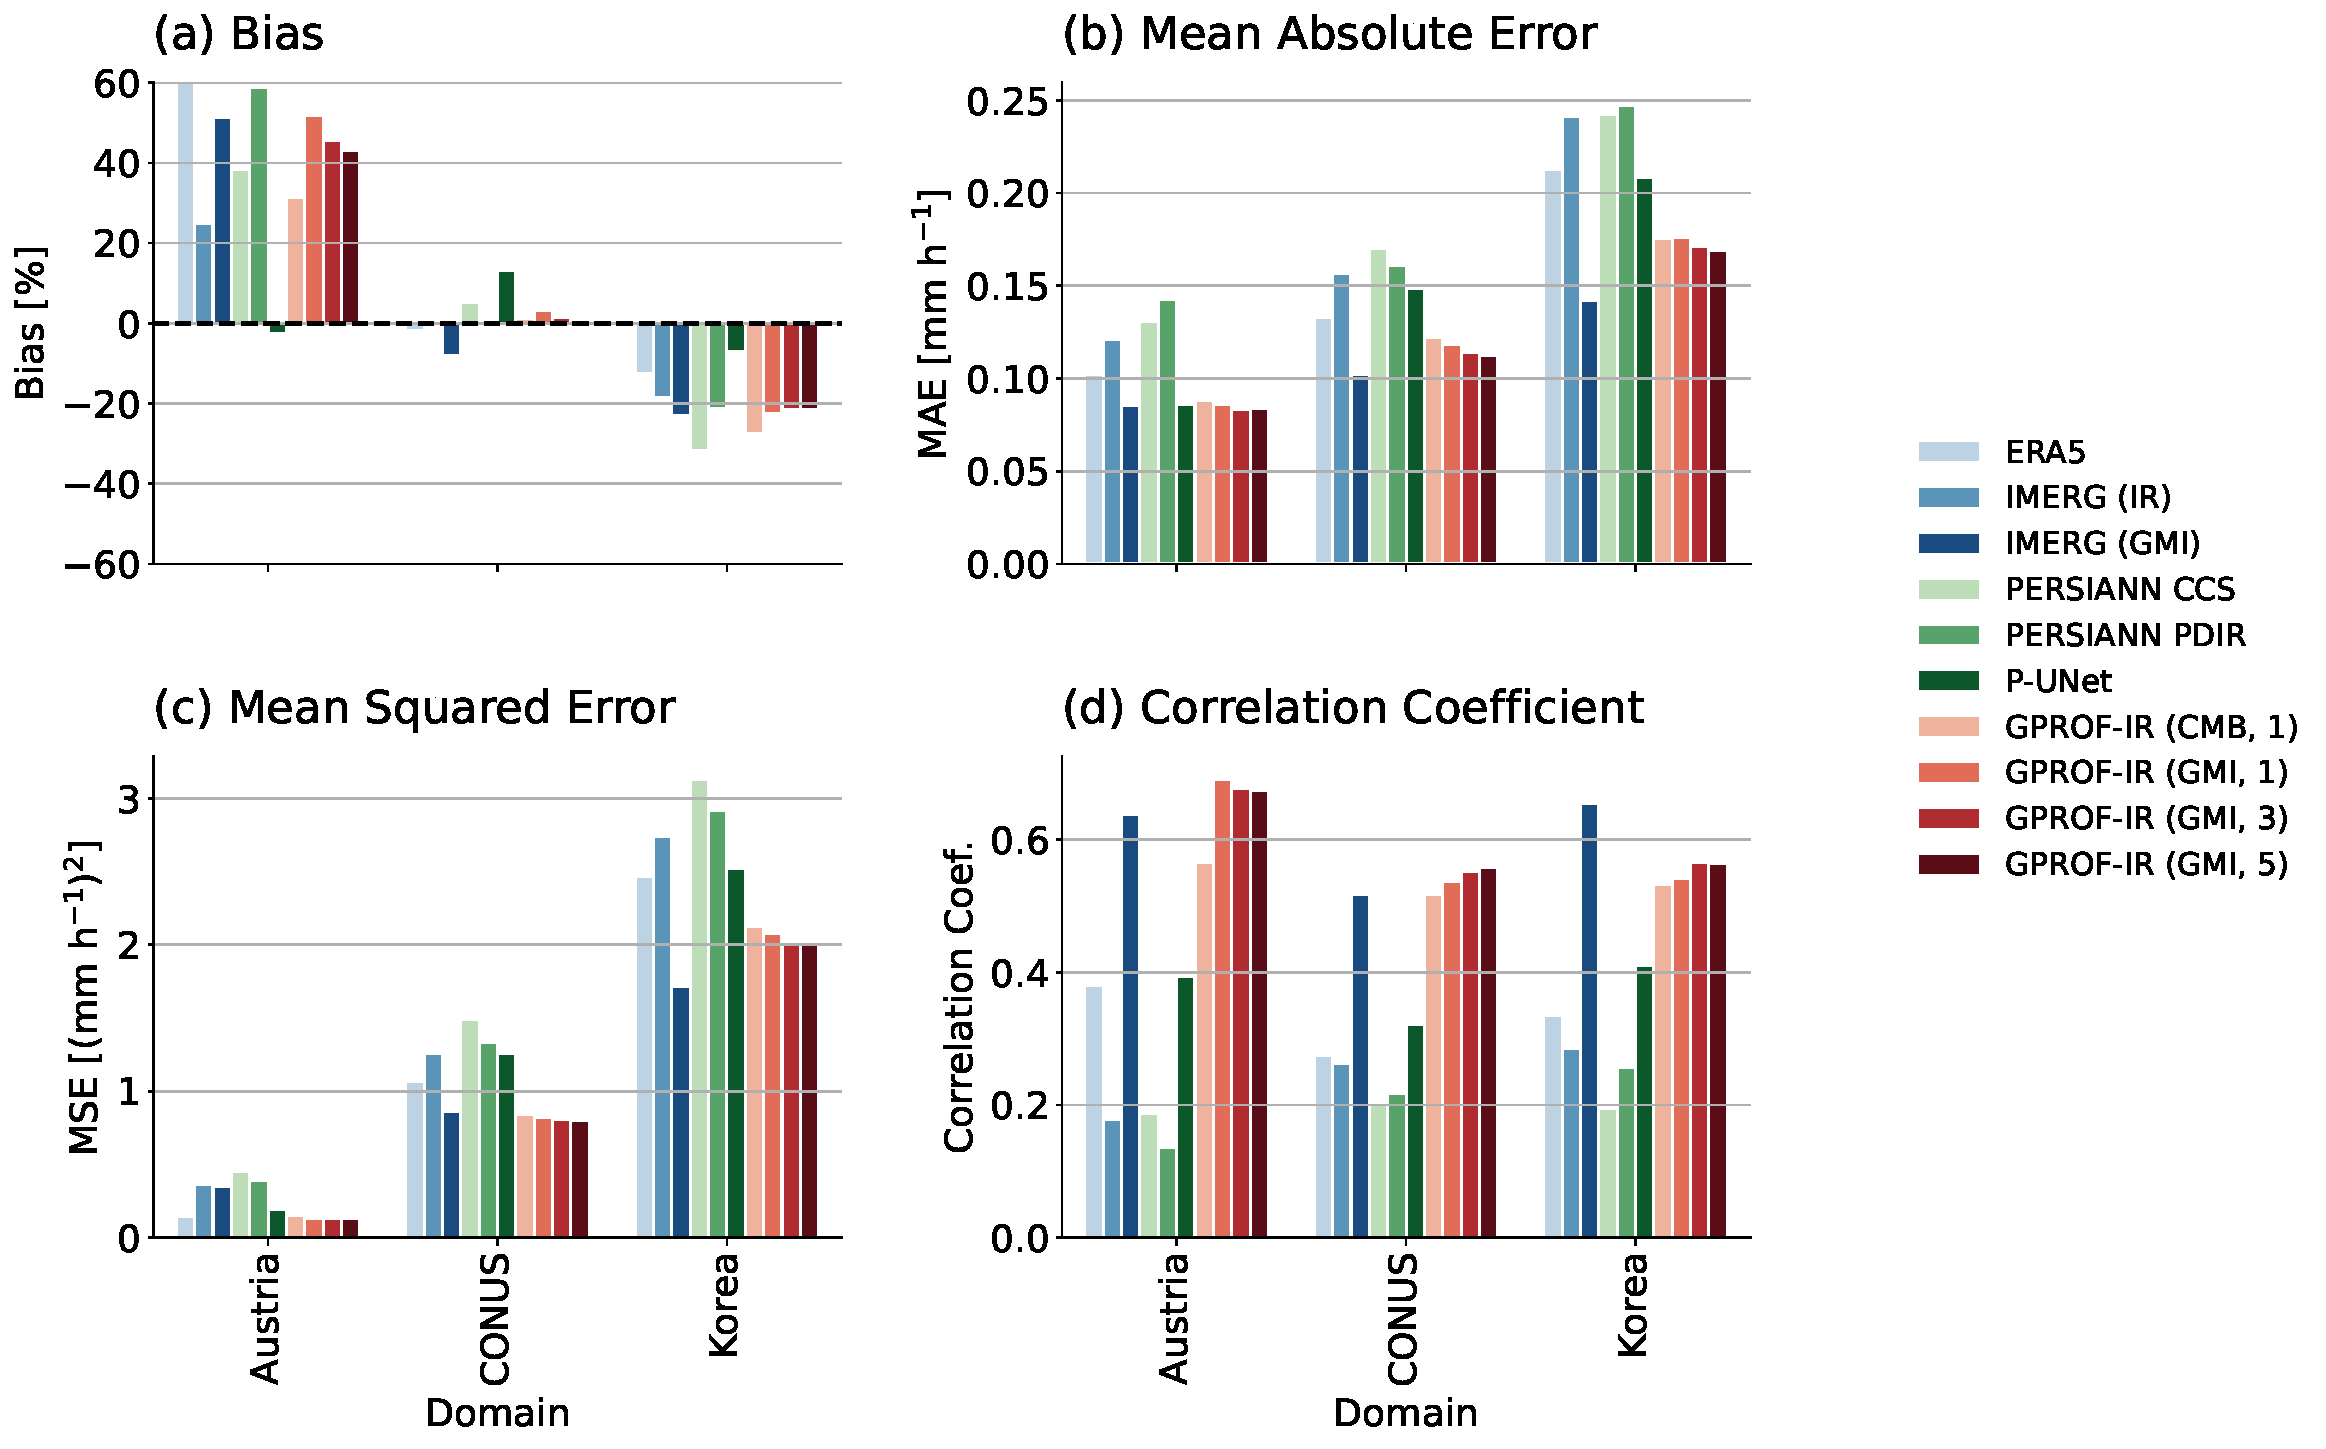
\includegraphics[width=37pc]{figures/figure07.pdf}}
 \caption{
  Spectral coherence curves for the GPROF-IR retrievals and baseline precipitation
  estimates assessed using the CONUS and Korea domains of the SatRain benchmark
  dataset. Panels (a) and (b) show the spectral coherence across scales in degree
  for the CONUS and Korea domains, respectively. Dashed black line marks the
  $\sqrt{\frac{1}{2}}$ threshold used to define the effective resolution of the precipitation
  estimates.
 }\label{fig:spectral_coherence}
\end{figure}

\paragraph{Precipitation Detection}

Figure~\ref{fig:precipitation_detection} assesses the skill of the GPROF-IR
retrievals to detect precipitation and heavy precipitation. Thresholds of 0.1 mm
h$^{-1}$ and 10 mm h$^{-1}$ are used to identify precipitation and heavy
precipitation, respectively. For the GPROF-IR retrievals, two different
detection approaches are compared: The first approach (red shading) is to use
the precipitation rate corresponding to the mean of the posterior distribution,
which is provide as the principal quantitative precipitation output from the
retrieval. The second approach is to use the probabilistic output of the model
to calculate the probability of the observed precipitation rate to exceed the
respective threshold (green shading) and use a detection threshold of 0.5
as a detection criterion.

Using the retrieved GPROF-IR precipitation rate to detect precipitation yields
slightly better detection skill than the IMERG IR and ERA5 baselines but remains
lower than the dection skill of the IMERG GMI estimates. The detection skill is
improved substantially when exceedance probabilities are used instead of
precipitation rates. Using a detection threshold of 0.5, all GPROF-IR
configurations yield higher precipitation detection accuracy than IMERG GMI
across all testing domains. For precipitation detection, the GPROF-IR (CMB, 1)
configuration performs best among the GPROF-IR configuration, which is in
contrast to the relative performance found for precipitation quantification.

For the detection of heavy precipitation over CONUS, using the GPROF-IR
precipitation rates yields better detection skill than the IMERG GMI estimates
but the detection skill is further improved when the probabilistic GPROF-IR
output is used. Over the Korea domain, only the probabilistic GPROF-IR (CMB, 1)
configuration yields higher detection skill than IMERG GMI. Over Austria only
the IMERG GMI retrieval shows marginal skill, which is likely becuase of these
events occurring too infrequently over the domain.


\begin{figure}[h]
 \centerline{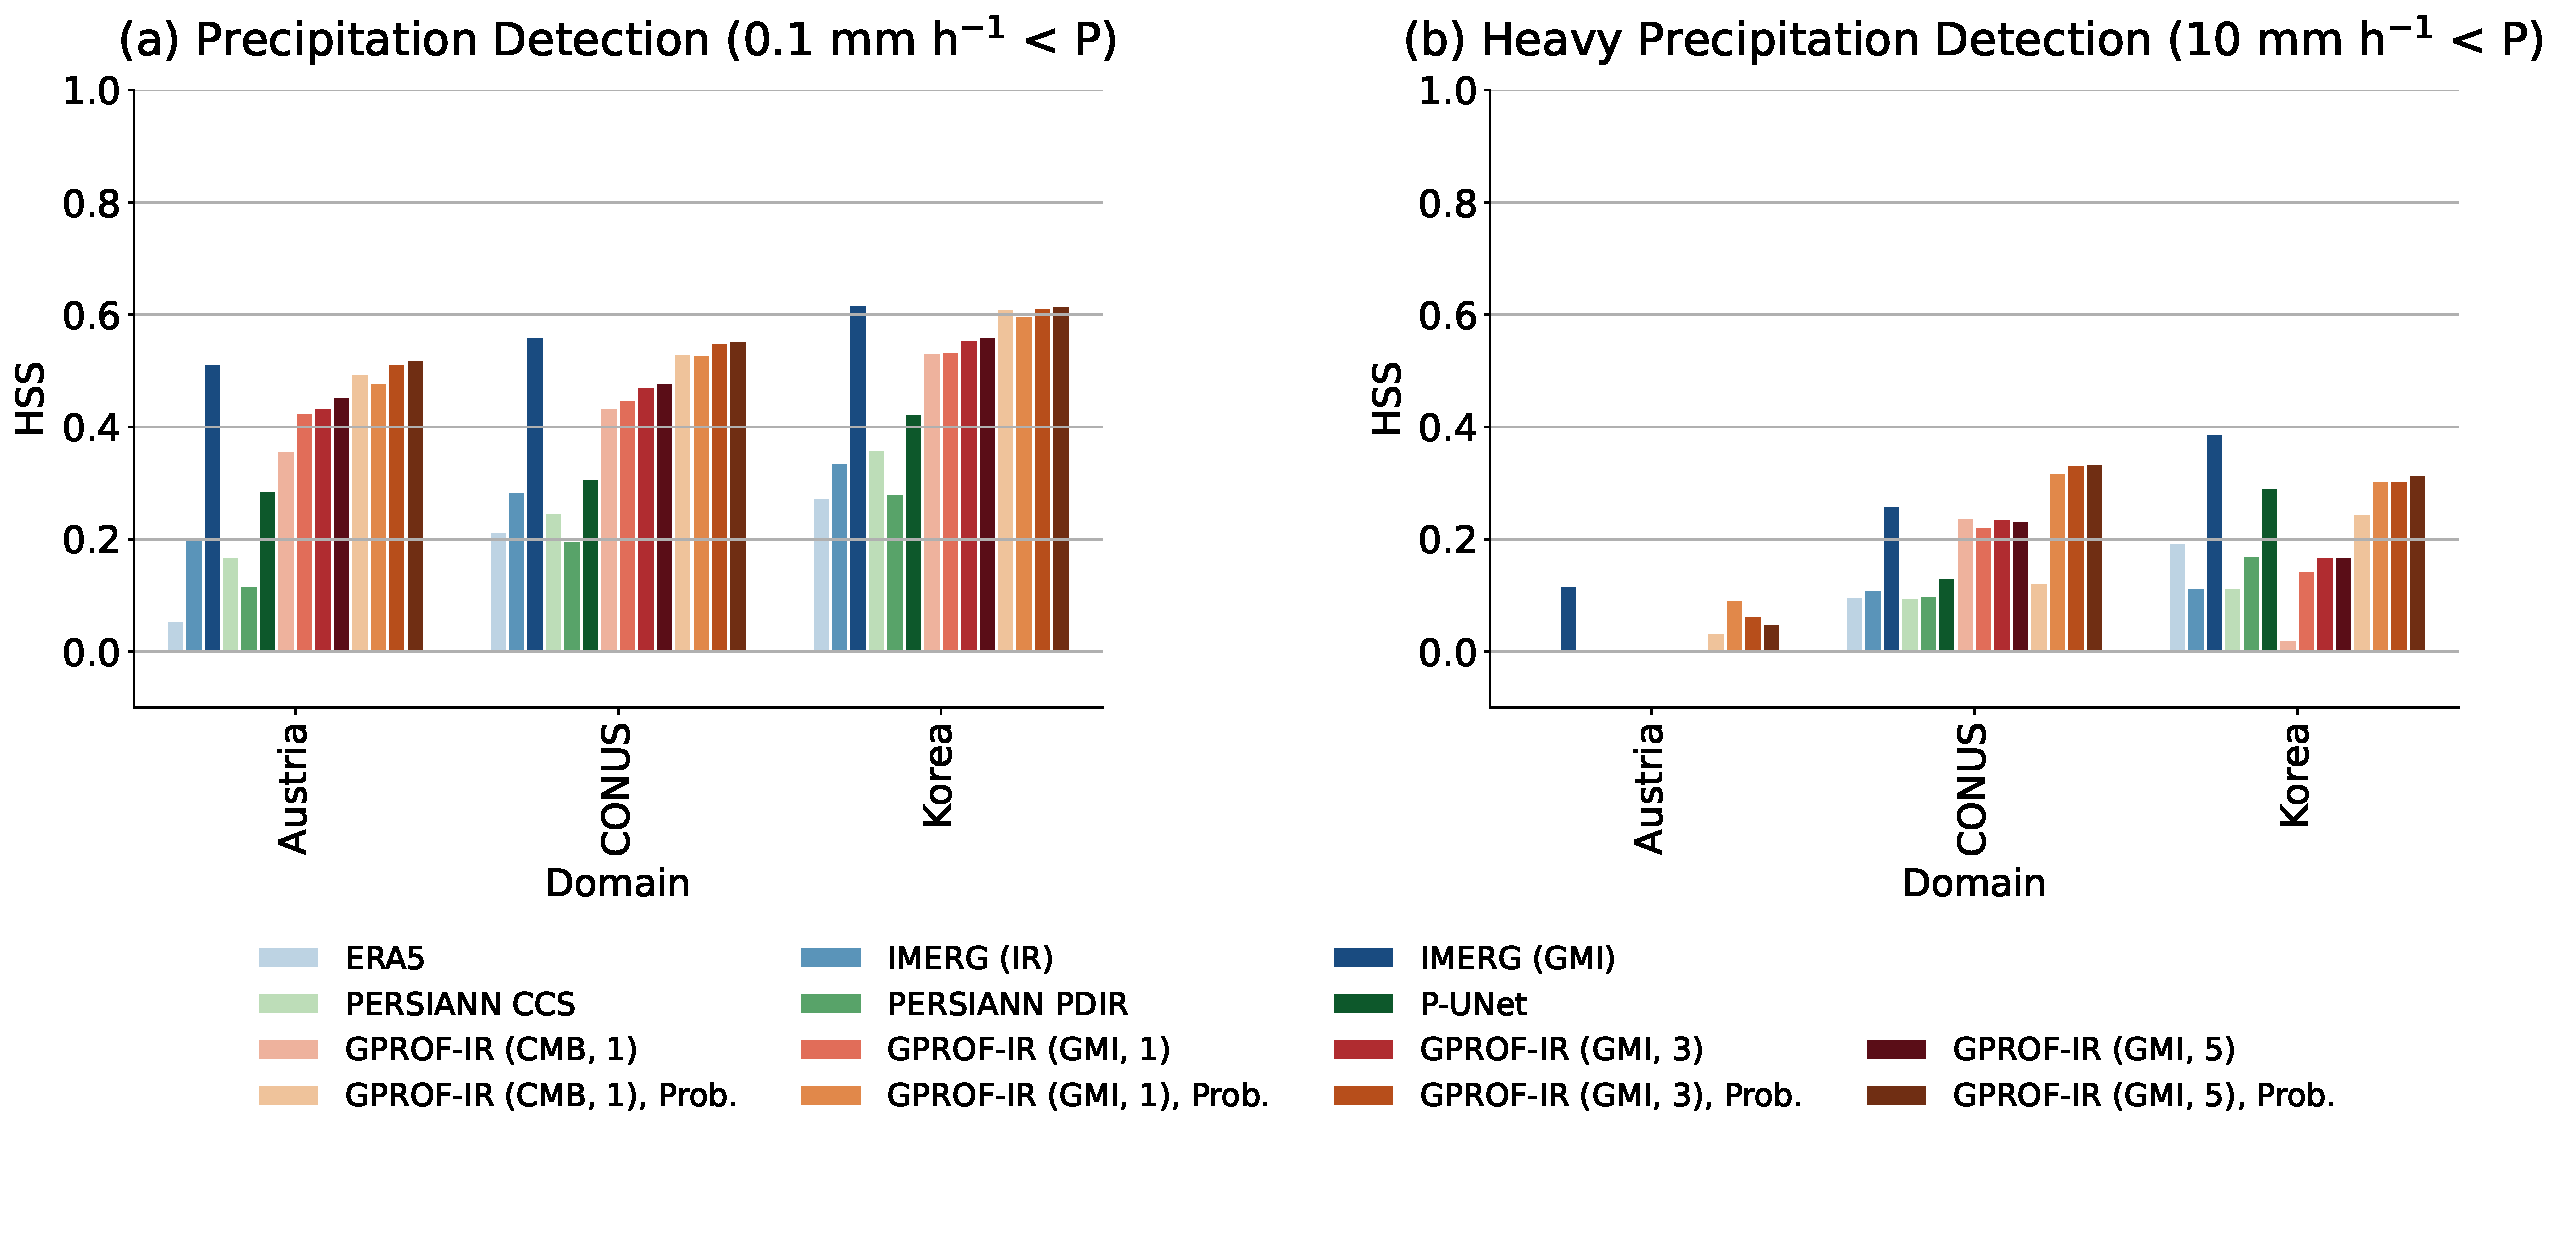
\includegraphics[width=37pc]{figures/figure08.pdf}}
 \caption{
   Detection skill for precipitation and heavy precipitation assessed on the SatRain benchmark dataset.
   Panel (a) shows the Heidke Skill Score (HSS) for the detection of precipitation (defined as any grid point
   exceeding $0.1$ mm h$^{-1}$). Panel (b) shows the corresponding results for the detection of heavy
   precipitation (defined as grid points exceeding 10 mm h$^{-1}$). Results for the GPROF-IR are presented
   using the retrieved precipitation rate as detection criterion (red shades) and using the probabilistic
   output to calculate exceedance properties and using a detection threshold of 0.5.
 }\label{fig:precipitation_detection}
\end{figure}

To investigate the higher skill of the GPROF-IR (CMB, 1) configuration for
precipitation detection, the probabilistic detection skill is assessed using
precision and recall curves in Fig.\ref{fig:precision_recall}. Despite yielding
higher HSS, the precision-recall cuve of the GPROF-IR (CMB, 1) retrieval stays
below that of the other configurations for both precipitation detection and
heavy precipitation detection, indicating that its detection skill across
detection thresholds is in fact lower than that of the other configurations. The
filled marker in each plot marks the precision and recall for the detection
threshold of 0.5 used for the results in Fig.~\ref{fig:precipitation_detection}.
The 0.5 threshold is systematically located at lower recall and higher precision
for the GPROF-IR (CMB, 1) configuration than for the GPROF V08 GMI based
retrievals. The higher HSS scores for the GPROF-IR (CMB, 1) retrieval are thus
not due a higher skill of the retrieval to detect precipitation or heavy
precipitation, but rather due to different detection characteristics resulting
from the use of 0.5 as detection threshold.

The GPROF-IR retrievals thus show similar skill for precipitation detection as
for precipitation quantification, when the statistical characteristics of the
retrieval output are taken into account. This further highlights that
detection-skill metrics should be used with caution to assess the skill of
precipitation retrievals.

\begin{figure}[h]
 \centerline{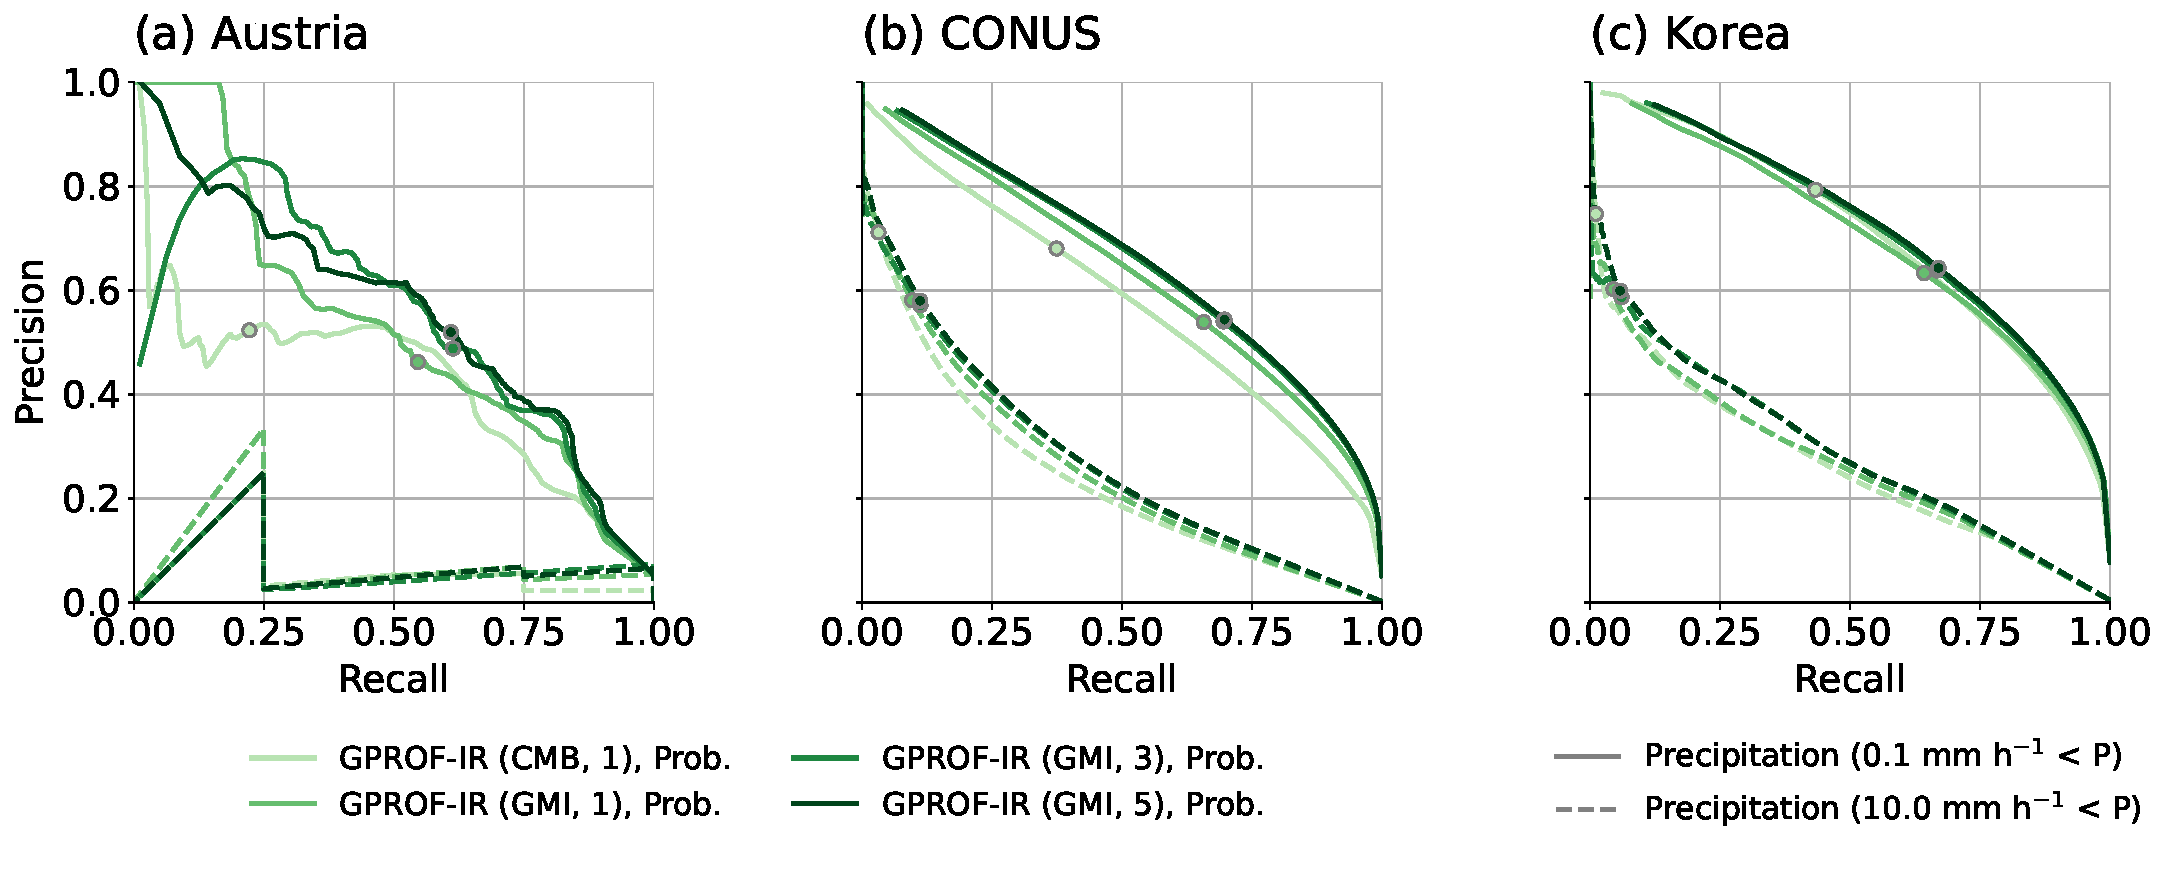
\includegraphics[width=37pc]{figures/figure09.pdf}}
 \caption{
   Precision recall curves for the probability of precipitation and probability of heavy precipitation outputs of
   the GPROF-IR retrievals. Filled markers show the reuslts obtained using a detection threshold of 0.5
   used to produce the results in Fig.~\ref{fig:precipitation_detection}
 }\label{fig:precision_recall}
\end{figure}

 \paragraph{Case Studies}

We further assess the accuracy of the GPROF-IR retrievals using two case studies
over the Korea and CONUS domains.

Figure~\ref{fig:case_study_1} shows reference and retrieved precipitation during
the landfall of Typhoon Khanun over the Korean peninsula \citep{bi_khanun_2025}.
The principal precipitation features in the reference precipitation field are
two strong cyclonic rain bands in the south-eastern quadrant of the domain as
well as strong convection in the north-eastern quadrant. The ERA5 estimates
capture the general cyclonic structure and the precipitation in the
north-eastern part of the scene but lack finer convective structures. The IMERG
GMI precipitation estimates yield the best agreement with the reference
estimates capturing the principal rain bands as well as the embedded convection.
The IMERG IR precipitation estimates, on the other hand, fail to reproduce the
structure of the cyclone. Although the estimates contain substantial small-scale
variability, it is unrelated to any of the fine-scale structures in the
reference data. The single-step GPROF-IR retrievals reproduce the large-scale
precipitation structures but also lack any of the finer embedded precipitation
structures. The inclusion of temporal information yields notable and visible
improvements with the retrieval being clearly able to reproduce more of the
embedded precipitation features and the negative bias being reduced from -38 \%
for the GPROF-IR (CMB, 1) retrieval to -14 \% for the GPROF-IR (GMI, 5)
retrieval.

\begin{figure}[h]
 \centerline{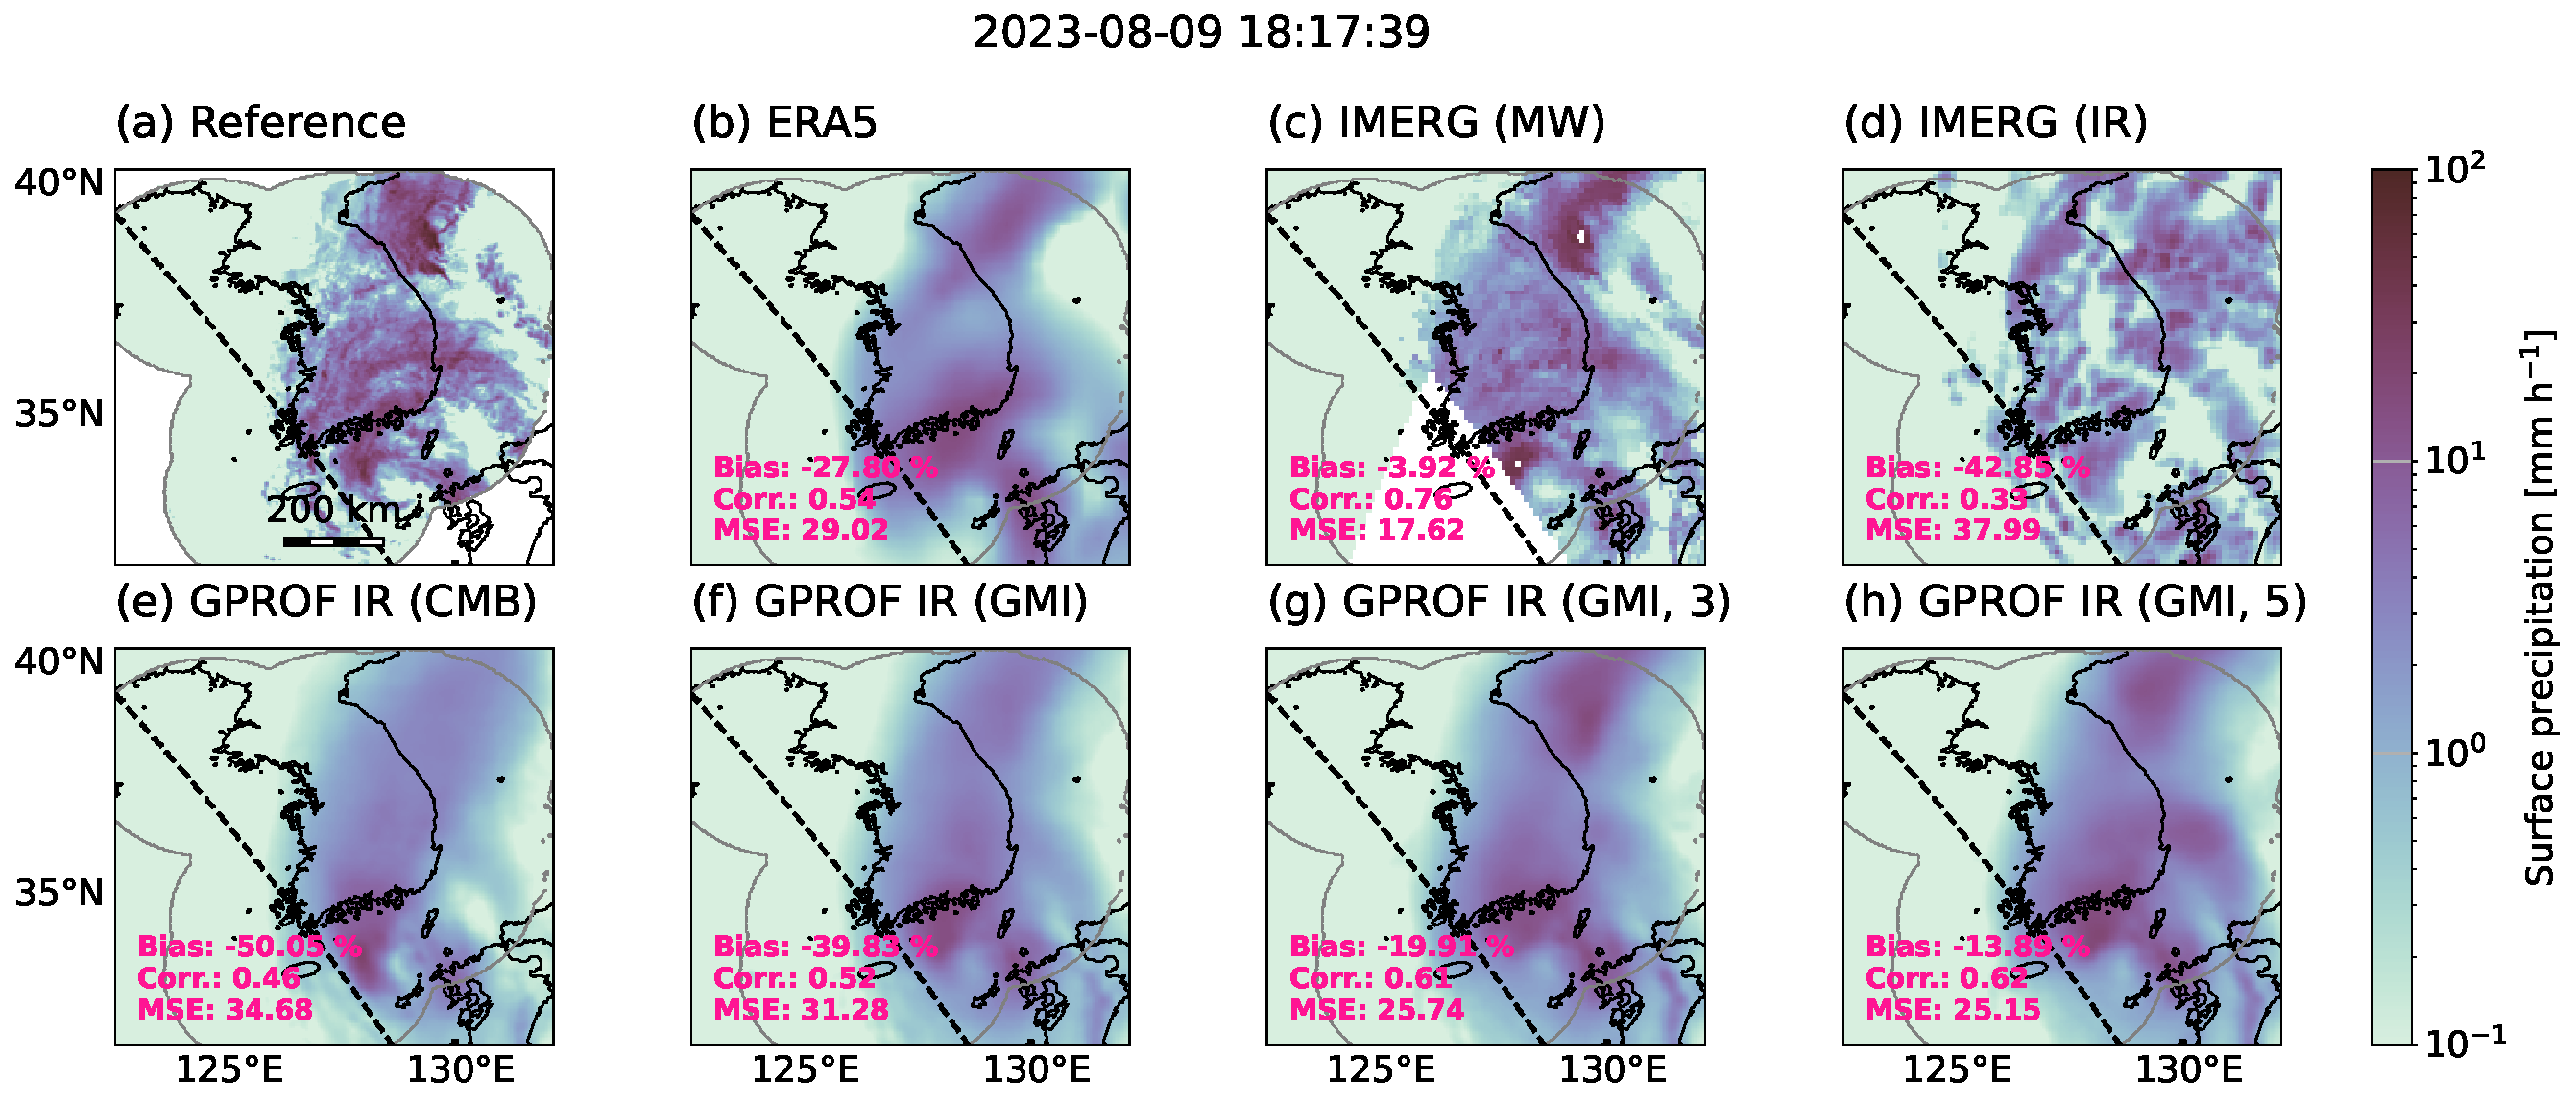
\includegraphics[width=37pc]{figures/figure10.pdf}}
 \caption{
    Reference and retrieved precipitation during landfall of Typhoon Khanun on the
    Korean peninsula. Panel (a) shows reference precipitation estimates from
    gauge-corrected ground-based radars from the SatRain benchmark dataset. Panels
    (b) – (h) show the results from the ERA5 and IMERG baselines as well as the
    GPROF-IR retrievals.
 }\label{fig:case_study_1}
\end{figure}

Figure~\ref{fig:case_study_2} shows a second case study over CONUS of a storm
system that spawned several tornados on April 12, 2022. The principal
precipitation features are a convective squall line in the south-western
quadrant and lighter, scattered precipitation in the north. For this case, the
ERA5 estimates show the worst agreement with the reference data. Although ERA5
captures some of the lighter precipitation in the North, it misplaces the
convection in the South and exaggerates its spatial extent. The IMERG GMI
estimates yield good agreement with the reference data capturing both the squall
line and the lighter precipitation. The IMERG IR estimates capture some of the
heavy convective precipitation but fail to reproduce the spatial organization of
the squall line. Furthermore, the light precipitation observed in the North
bears little resemblance with the reference data. The GPROF-IR retrievals yield
the best accuracy for this case study, accurately capturing the squall line
albeit slightly exaggerating its spatial extent. The GPROF-IR retrieval
overestimates the spatial coverage of precipitation in the North but generally
captures all of the important precipitation features visible in the reference
data.

The GPROF-IR retrieval performs well for this case study because IR brightness
temperatures are directly linked to intense precipitation on the ground.
Combined with the reduced information content in the PMW observations due to
background emission from the land surface, this likely explains GPROF-IR
retrieval is able to provide more accurate estimates than IMERG GMI for these
kind or precipitation regimes.

\begin{figure}[h]
 \centerline{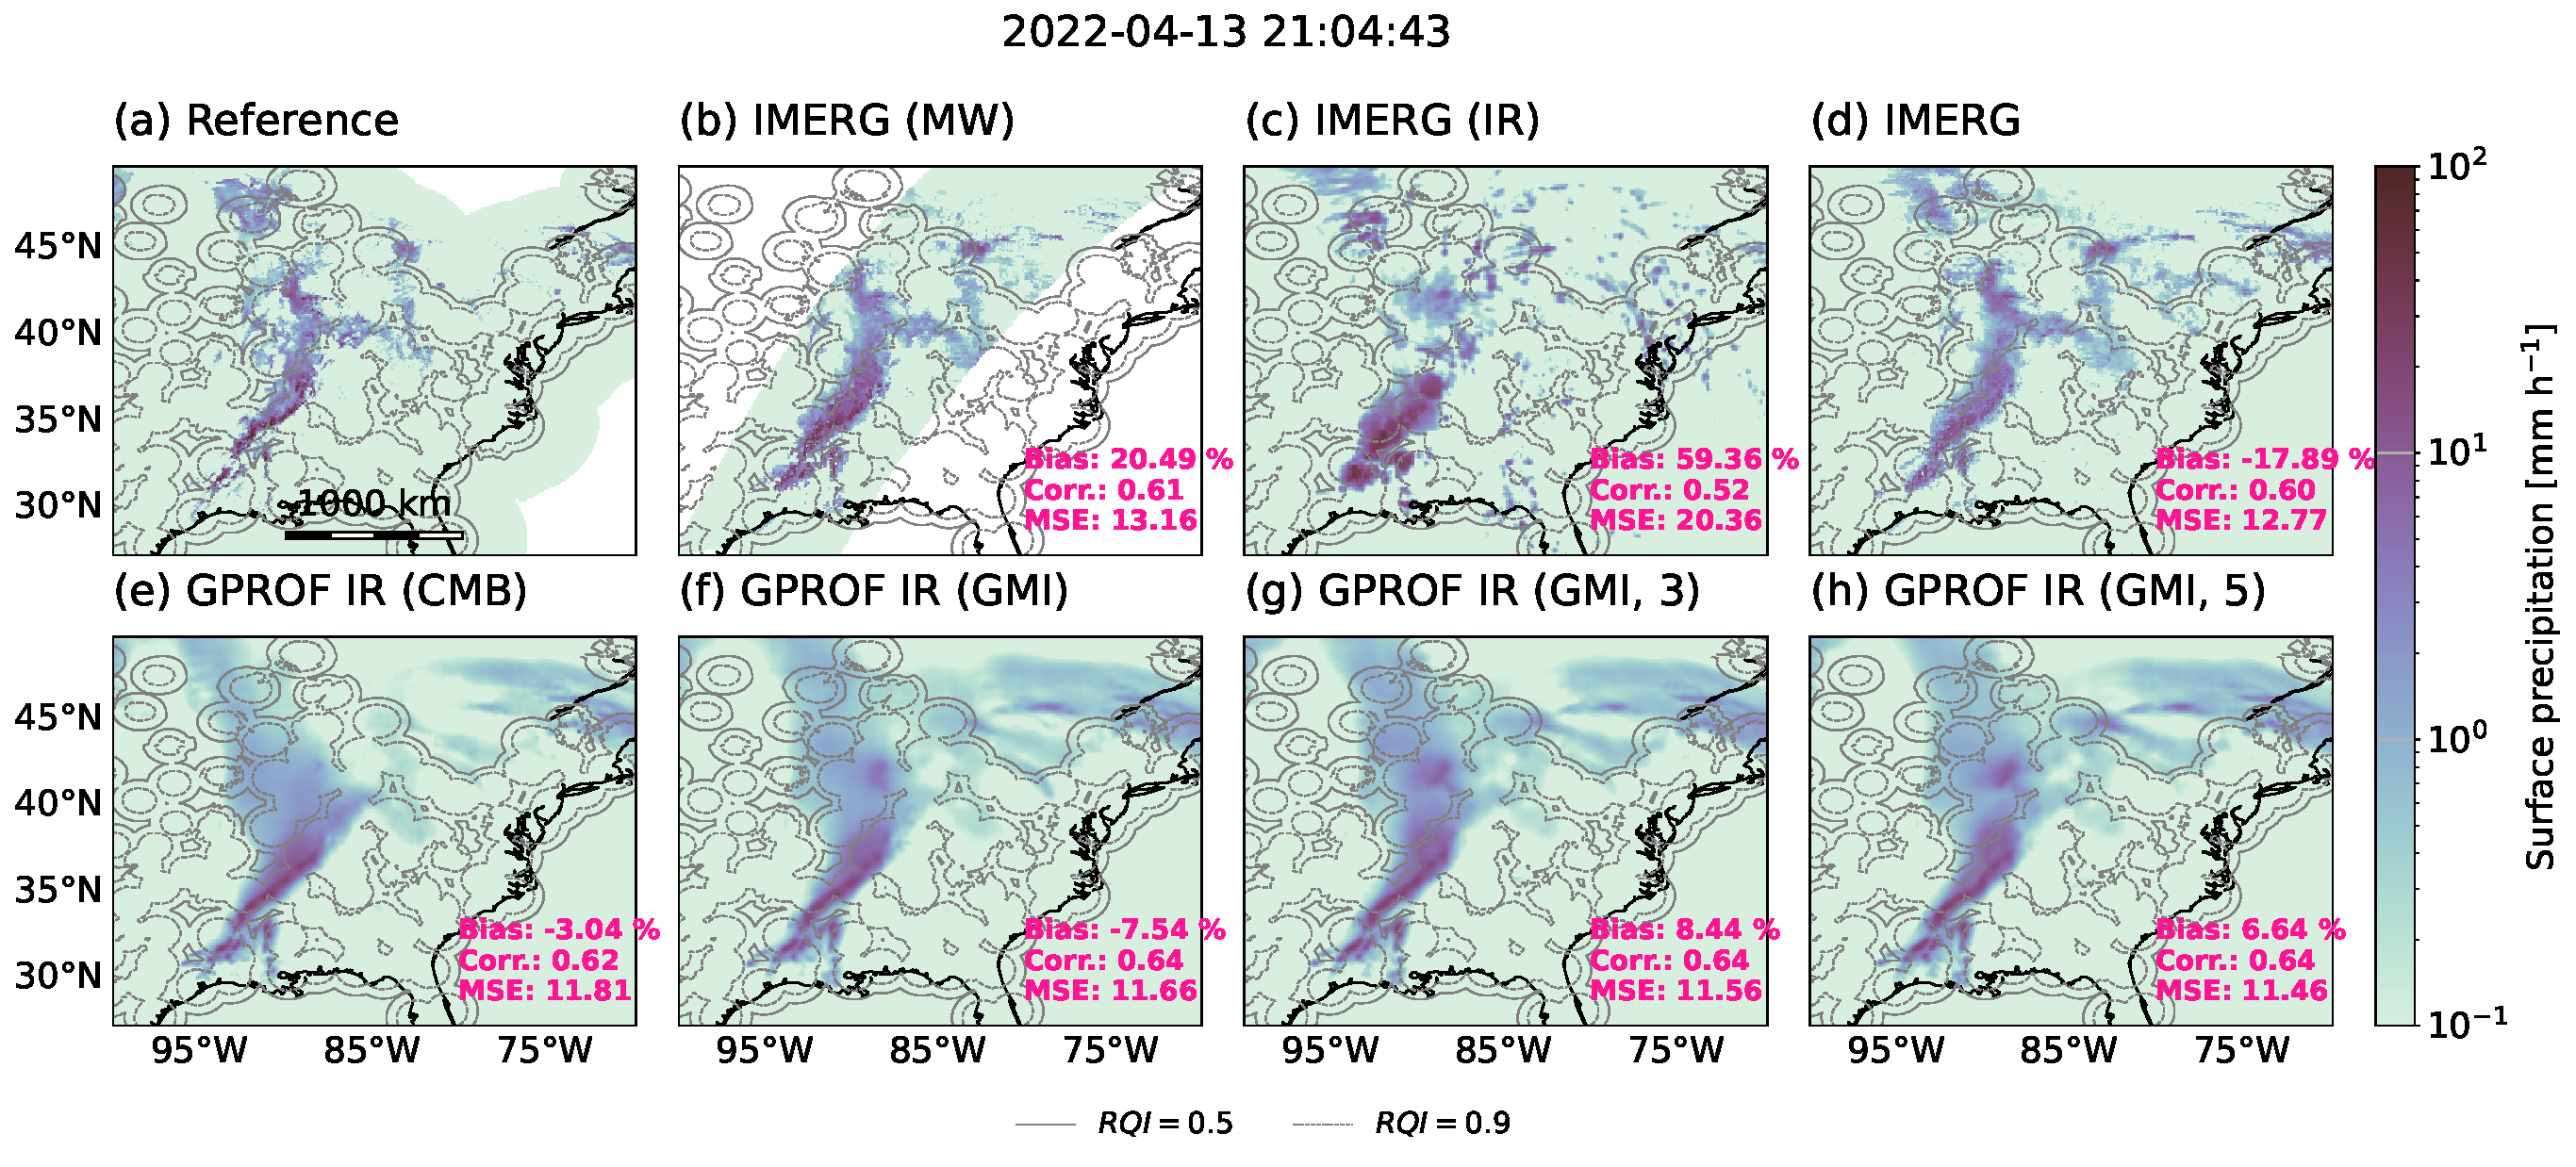
\includegraphics[width=37pc]{figures/figure11.pdf}}
 \caption{
    Reference and retrieved precipitation for a convective storms system on
    April 13, 2022 over CONUS. Panel (a) shows reference precipitation estimates
    from gauge-corrected ground-based radars from the SatRain benchmark dataset.
    Panels (b) – (h) show the results from the ERA5 and IMERG baselines as well
    as the GPROF-IR retrievals.
 }\label{fig:case_study_2}
\end{figure}

\subsubsection{OceanRAIN}

The validation using the SatRain dataset was largely limited to measurements
over land. To complement this land-focused validation, we also evaluate the GPROF-IR
(CMB, 1) and GPROF-IR (GMI, 3) retrievals against shipborne in-situ
precipitation measurements from the OceanRAIN dataset. The assessment focuses on
the GPROF-IR (GMI, 3) retrieval, which was selected as the preferred
configuration for operational processing as its accuracy is close to that of the
five-timestep configuration while requiring less input data. Additionally, we
include the GPROF-IR (CMB, 1) configuration to assess the impact of using GPROF
V08 GMI reference estimates as training targets. The GPROF V08 training data
uses the GPROF-NN XPR retrieval to fill in missing light precipitation in the 2BCMB
dataset over oceans. This has been shown to reduce systematic underestimation of
high-latitude and frozen precipitation \citep{pfreundschuh_xpr_2026}. However, the
analysis was limited to GMI overpasses over the OceanRAIN vessels. The continuous
availability of the IR observations thus provides an opportunity to indirectly
validate the representation of light and frozen precipitation in GPROF V08
retrievals using a much larger number of samples.

For the validation against shipborne distrometer measurements from the OceanRAIN
dataset, we have run the GPROF-IR (CMB, 1) and GPROF-IR (GMI, 3) retrievals for
the years 2017 and 2018. For each half-hourly timestep, the GPROF-IR
precipitation estimates were matched with half-hourly averages from the
OceanRAIN distrometer precipitation rates and corresponding IMERG results. The
summary statistics from the validation are shown in Fig.~\ref{fig:ocean_rain}.
For all match-ups, both IMERG and GPROF-IR retrievals have low biases while at
high-latitudes the GPROF-IR retrievals are biased low by 18\% for the GPROF
V08-based retrieval and 25\% for the 2BCMB-based retrieval. For frozen
precipitation the GPROF-IR (GMI, 3) retrieval achieves the lowest biases with
about 18\%, while the GPROF-IR (CMB, 1) retrieval is biased low by about 38\%.
This improved representation of high-latitude and frozen precipitation provides
further evidence that the GPROF-NN XPR retrieval can capture light and frozen
precipitation missed by GPM DPR-based precipitation estimates and thus
confirms the findings from the initial validation in \citet{pfreundschuh_xpr_2026}.

In terms of retrieval error, the validation against shipborne measurements shows
results similar to those obtained over land. The GPROF-IR retrievals
substantially improve upon the IMERG IR precipitation estimates, yielding
results comparable to the merged IMERG estimates and even outperforming them at
high latitudes and for frozen precipitation. It should be noted that unlike the
validation on the SatRain dataset, which was limited to GMI overpasses, this
analysis uses the merged IMERG precipitation estimates from all half-hourly
timesteps during the validation period. The IMERG results shown here are
therefore more representative of the average IMERG accuracy rather than the
best-case accuracy during GMI overpasses.

\begin{figure}[h]
 \centerline{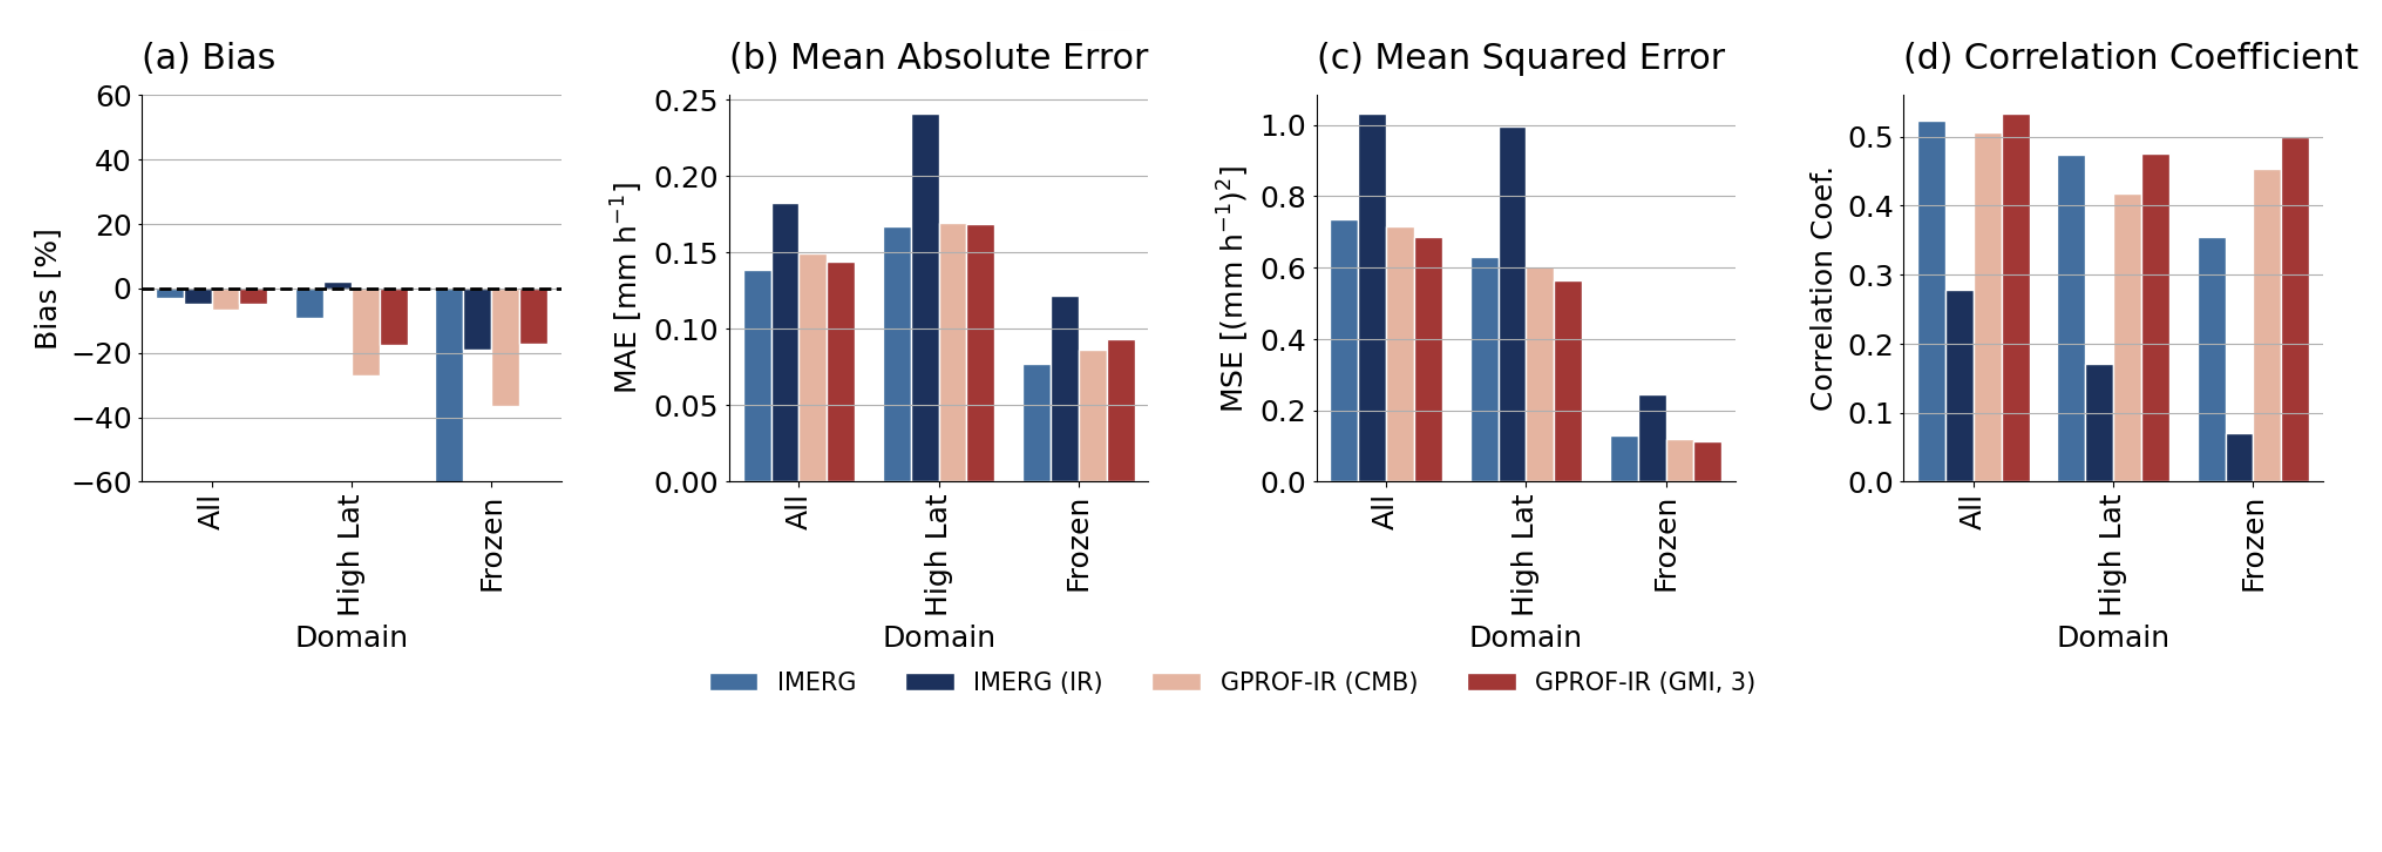
\includegraphics[width=37pc]{figures/figure12.png}}
 \caption{
GPROF-IR retrievals from the years 2017 and 2018 assessed against shipborne
distrometer measurements from the OceanRAIN dataset. Panels (a) – (d) compare
bias, mean absolute error, mean squared error, and correlation coefficient of
the two of GPROF-IR configurations against IMERG baseline estimates. Each panel
shows results for all matchups, high-latitudes (poleward of 45$^\circ$), and with and for
mixed and frozen precipitation.
 }\label{fig:ocean_rain}
\end{figure}


\subsection{Precipitation Climatology}

 Below we characterize global precipitation climatologies of the
GPROF-IR (GMI, 3) configuration derived from from the year 2022 to corresponding
estimates from principal precipitation datasets. To reduce diffences due to
different spatiotemporal sampling of the datasets, we extract precipitation
estimates from GPROF-IR, ERA5, and GPCP matching the observations of GPROF V08
GMI retrievals.

Figure~\ref{fig:zonal_means} shows zonal means from the GPROF-IR (GMI, 3)
retrieval compared to corresponding estimates from GPROF V08 GMI, ERA5 and GPCP.
As expected, GPROF-IR results closely track the GPROF reference estimates over
both ocean and land. Over ocean, all datasets agree well over the tropics and
subtropics but start to diverge at higher latitudes. Over northern hemisphere
oceans, the GPROF V08 GMI, GPROF-IR and ERA5 means show close agreement while
the GPCP estimates are notably higher. Over the southern hemisphere ocean, the
GPROF V08 GMI and GPROF-IR estimates lie between the ERA5 and GPCP estimates at
around 40$^\circ$ S but fall below the ERA5 estimates poleward of 50$^\circ$ S. Over
land, the discrepancies between the datasets are larger. Both GPCP and ERA5 are
about 20\% higher over tropical land. Over northern hemisphere land, the GPROF V08,
GPROF-IR, and GPCP estimates agree well while ERA5 yields slightly higher
average precipitation rates. Over southern hemisphere land, the differences are
much larger with GPCP being substantially lower than GPROF V08 and GPROF-IR and
ERA5 being substantially higher. However, these differences may be enhanced by
the smaller sample size due to lower land coverage at these latitudes.

\begin{figure}[h]
 \centerline{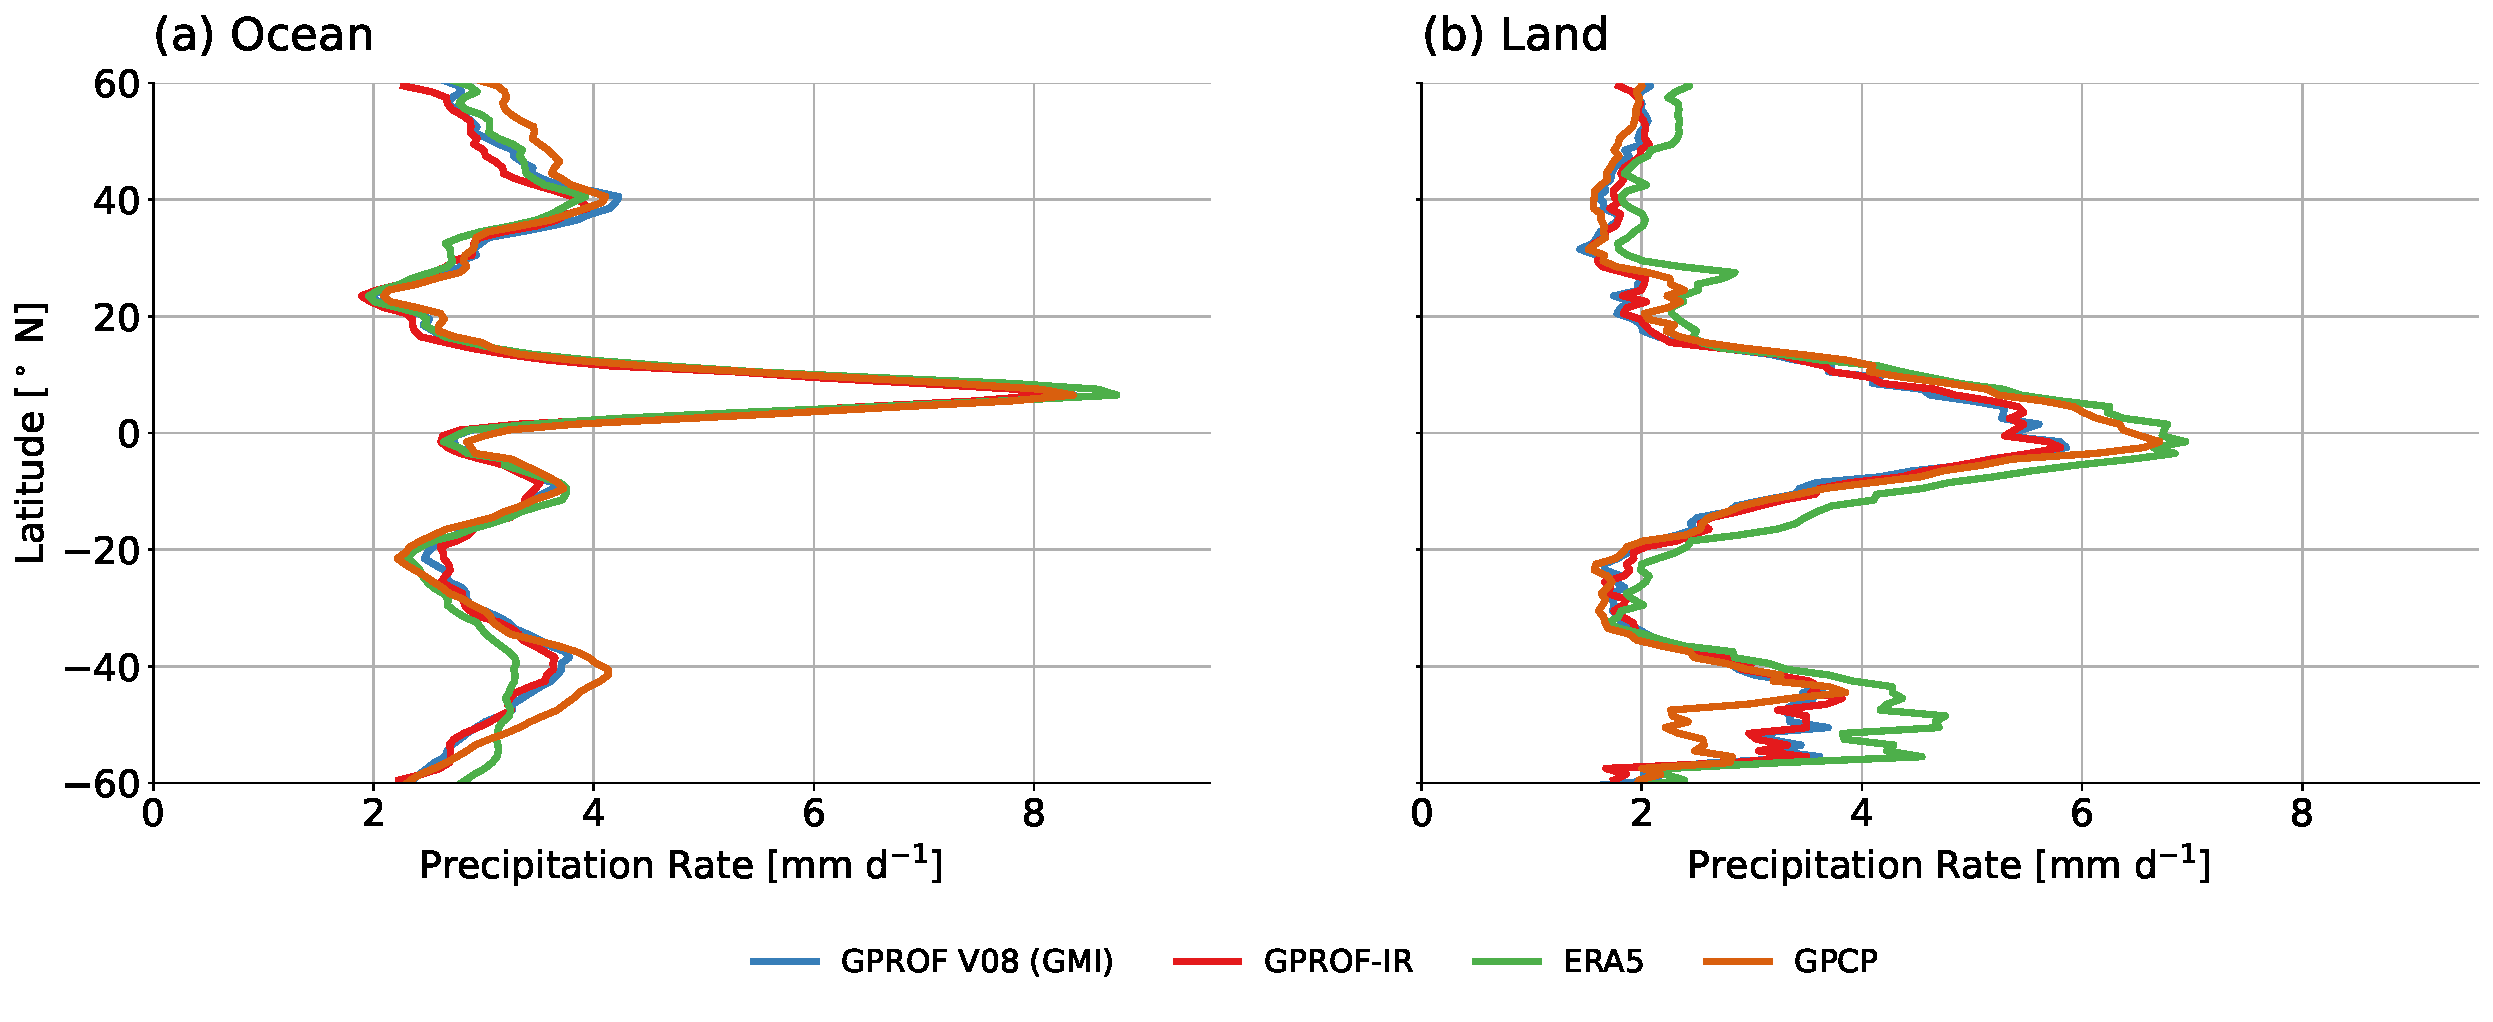
\includegraphics[width=37pc]{figures/figure13.pdf}}
 \caption{
    Zonal mean precipitation from GPROF V08, GPROF-IR, ERA5 and GPCP for 2022. Panel
    (a) displays the means for precipitation over oceans; panel (b) the means for
    precipitation over land.
 }\label{fig:zonal_means}
\end{figure}

Figure~\ref{fig:means} shows the global precipitation distributions for GPROF
V08, GPROF-IR, ERA5, and GPCP. The distribution of the GPROF-IR estimates
closely resembles that of GPROF V08. Differences between GPROF V08 and GPROF-IR
are mostly irregularly distributed and don’t exhibit any notable spatial
patterns, indicating that they are largely driven by random retrieval errors for
individual precipitation events. Both ERA5 and GPCP show larger systematic
differences particularly over land. ERA5 tends to be higher over land than both
GPROF V08 and GPROF-IR, particularly in the tropics. For GPCP the differences are
less uniform with regions of both underestimation and overestimation present at
all latitudes.

The GPROF-IR (GMI, 3) retrievals largely reproduce the distribution of GPROF
V08. Since the GPROF-IR retrieval is designed to provide background
precipitation estimates to be merged with GPROF V08 retrievals, the
climatological consistency constitutes an additional desirable feature of the
GPROF-IR retrievals.

\begin{figure}[h]
 \centerline{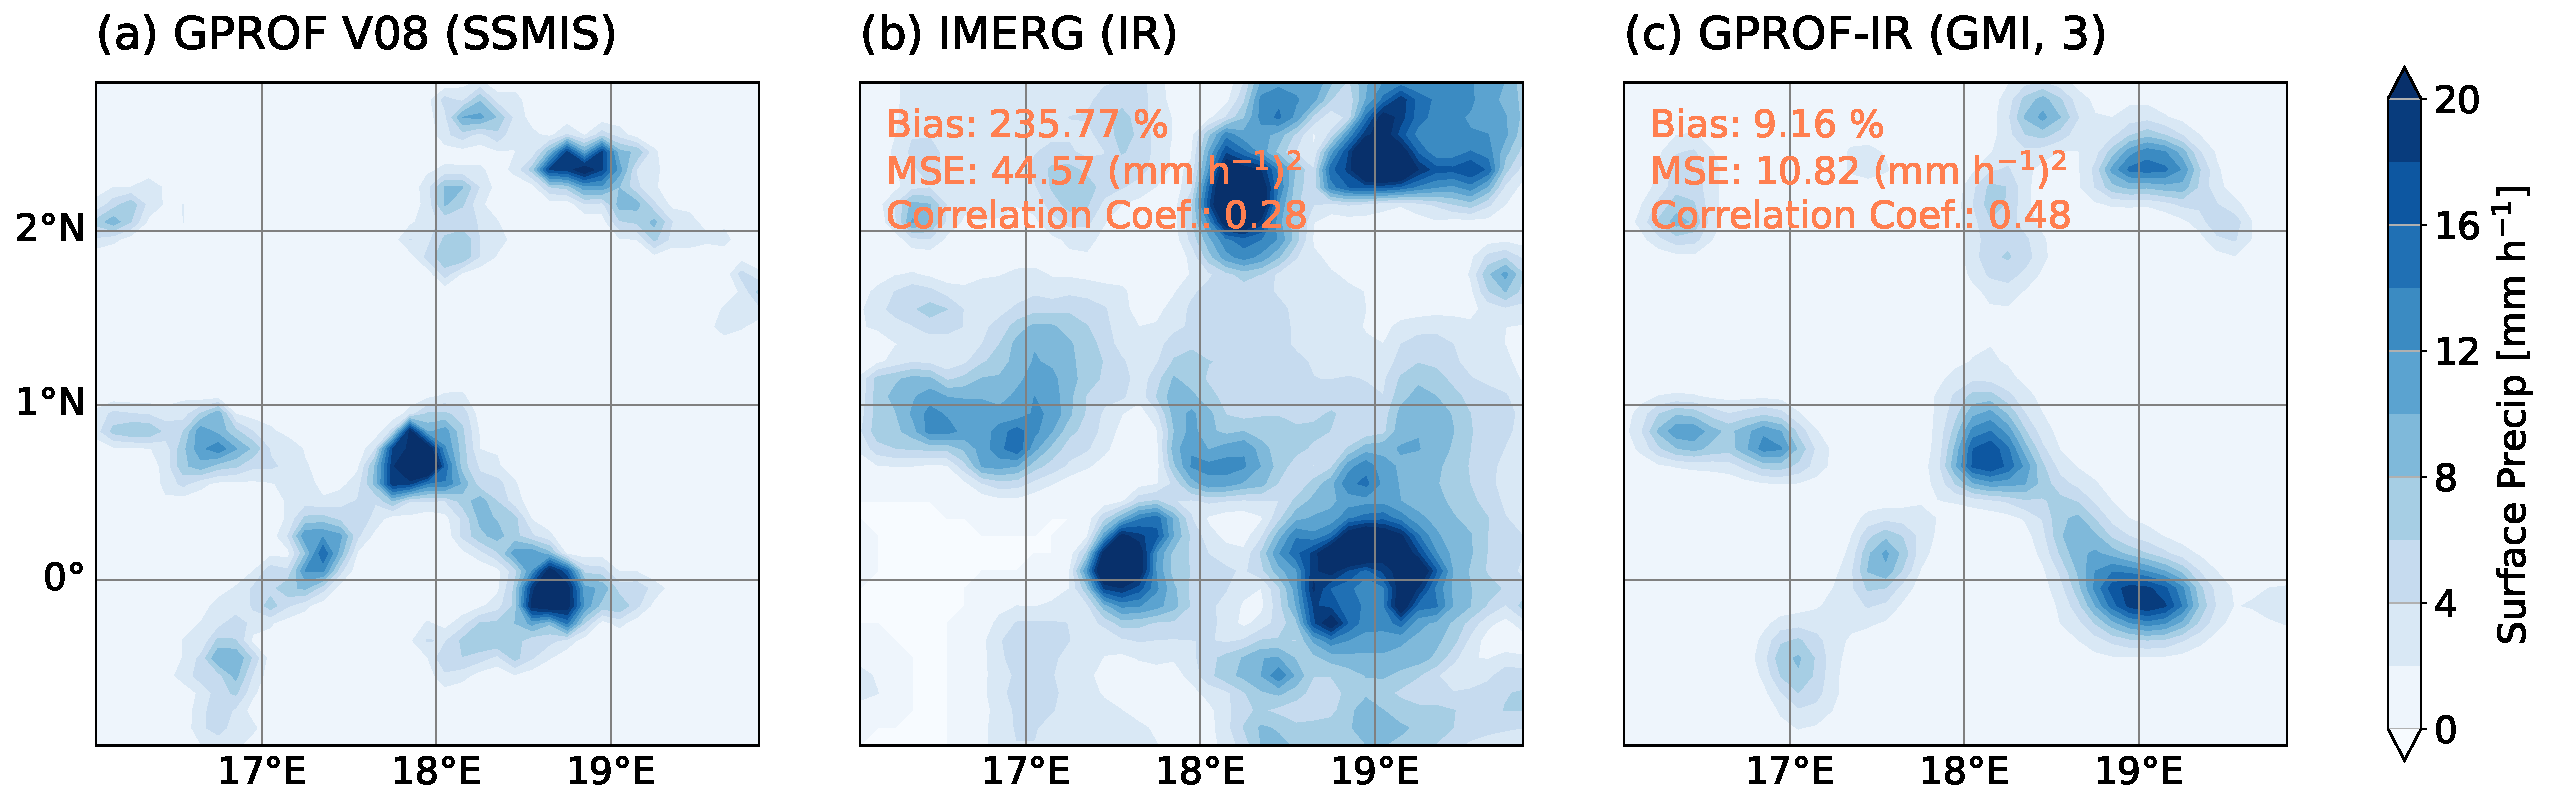
\includegraphics[width=37pc]{figures/figure14.pdf}}
 \caption{
Global precipitation distributions from GPROF V08, GPROF-IR, ERA5, and GPCP for
2022. The first column displays the average precipitation distributions; the
second column displays the difference with respect to GPROF V08.
 }\label{fig:means}
\end{figure}

\section{Summary and Conclusions}
\label{sec:summary_and_conclusions}

This study developed and validated GPROF-IR — a novel single-channel IR
precipitation estimation algorithm to provide background precipitation estimates
for merged satellite precipitation datasets. The retrieval leverages a CNN and
temporally resolved input observations allowing it to considerably improve upon
conventional IR precipitation retrievals. Despite using only single-channel IR
observations, GPROF-IR achieves higher accuracy than IMERG precipitation
estimates during GMI overpasses over CONUS and continental Europe. Since
geostationary IR observations are available around much of the globe every 30
min, the ability of GPROF-IR to provide more accurate precipitation estimates
than the much less frequent PMW obverpasses constitutes a major advancement for global
precipitation monitoring. However, it should also that the next operational
version of GPROF -- GPROF V08 -- will use a similar CNN-based retrieval that has
been shown to markedly improve PMW retrievals as well.

Validation against independent precipitation estimates over the Korean peninsula
and the global oceans showed that the accuracy approaches but remains below that
of conventional PMW retrievals over water surfaces and precipitation regimes
dominated by shallower precipitation systems. Nonetheless, the GPROF-IR yields
notable improvements over conventional IR retrievals,  reducing
mean absolute and mean square error and doubling the linear correlation
coefficient across a variety of precipitation regimes.


\subsubsection{Consequences for ML Precipitation Retrieval Design}

GPROF-IR is the first global single-channel IR retrieval to achieve higher
accuracy than IMERG PMW precipitation estimates over continental landmasses,
establishing a new state of the art for this class of methods. This is
corroborated by comparisons with IR-based precipitation products from the
PERSIANN family \citep{hong_ccs_2004, nguyen2020persiann, nguyen_punet_2026} shown in
Fig.~\ref{fig:evaluation_persiann}. Since PERSIANN products
are only available as hourly accumulations, their accuracy will be slightly
reduced  when evaluated against the SatRain reference data, which is
based on 2- and 10-minute radar observations over CONUS and Korea and
half-hourly accumulations over Austria. Nevertheless, the assessment on the
SatRain data reproduces relative accuracy of the PDIRNow, PU-Net, and IMERG
retrievals reported in \citet{nguyen_punet_2026} indicating that the assessment
in Fig.~\ref{fig:evaluation_persiann} remains representative.
\begin{figure}[h]
 \centerline{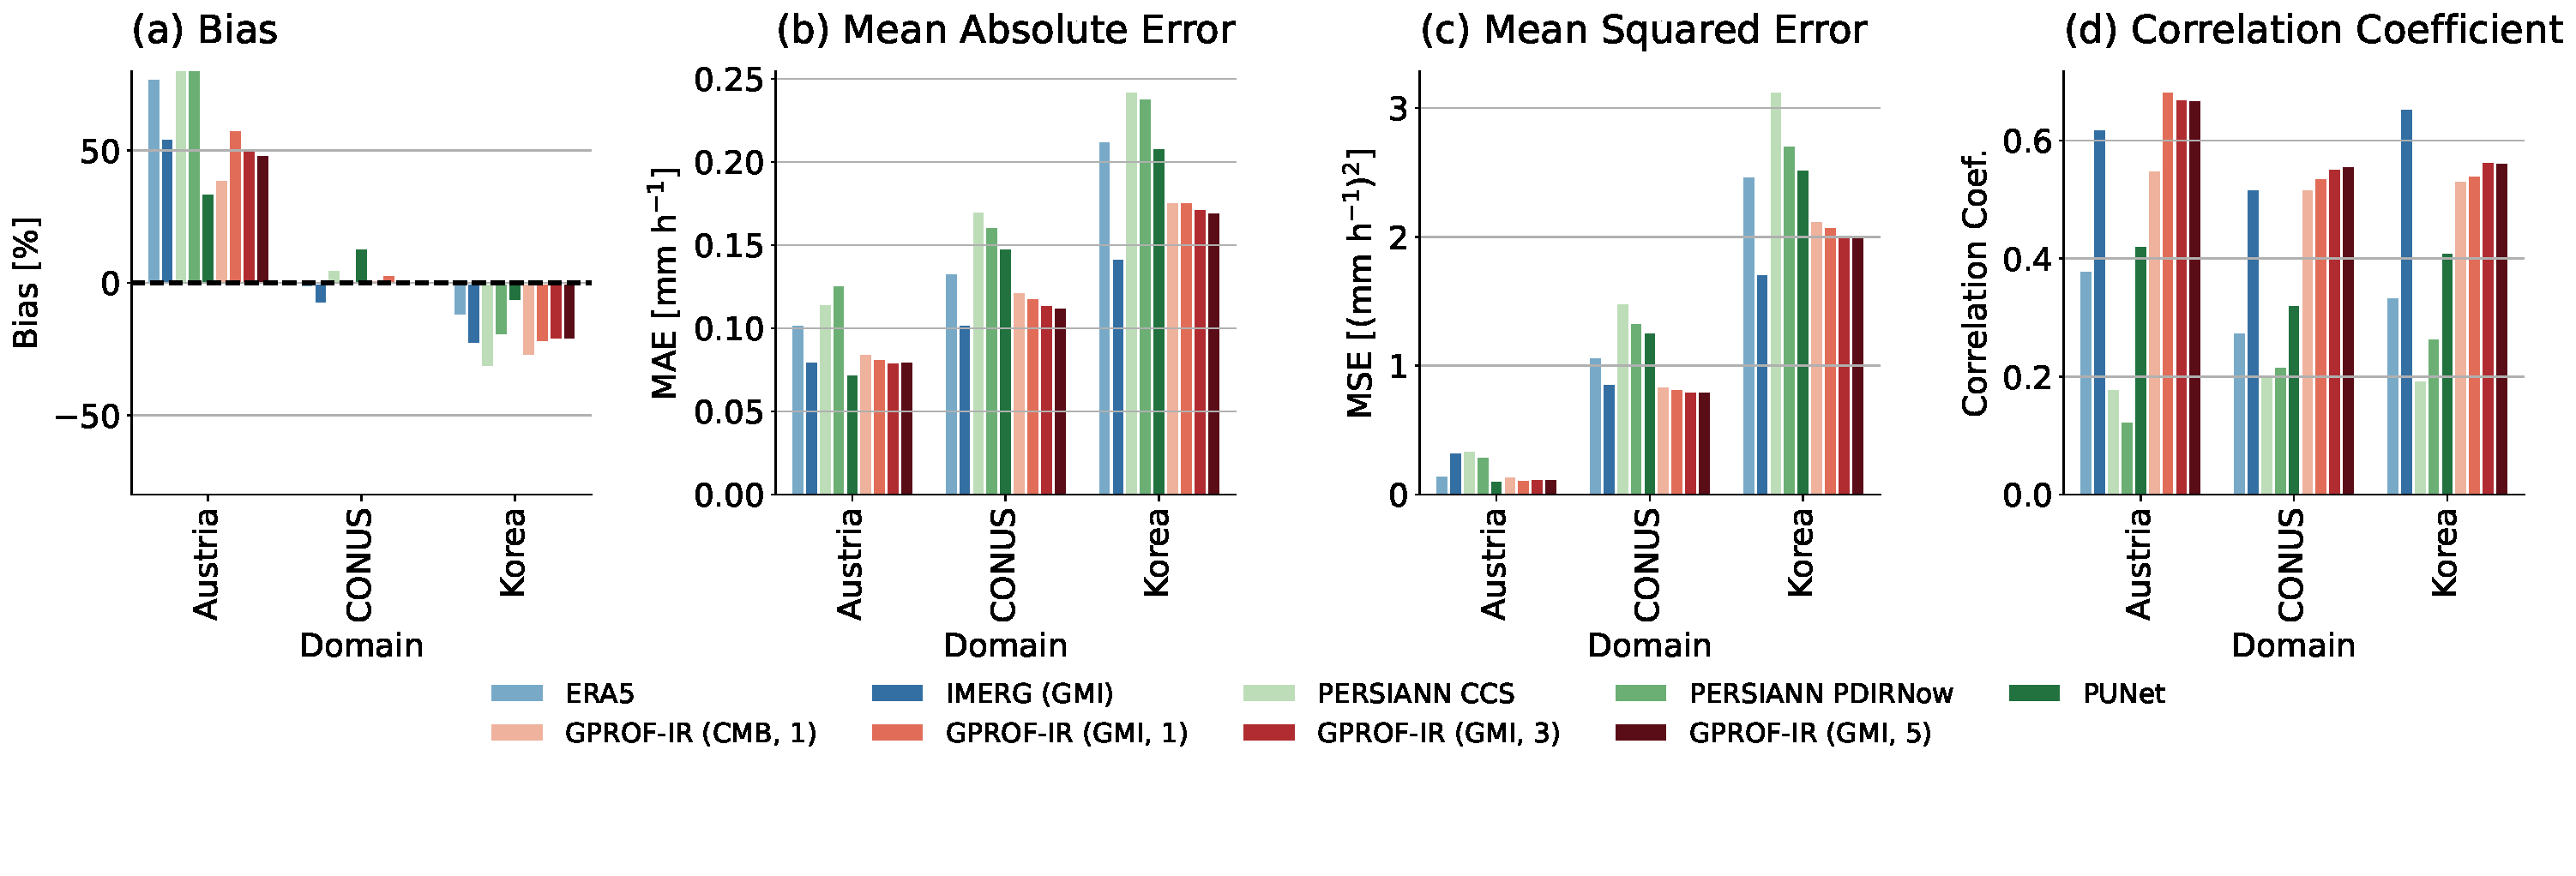
\includegraphics[width=37pc]{figures/figure15.pdf}}
 \caption{
   Comparison of GPROF-IR and PERSIANN IR precipitation products using the SatRain
   benchmark dataset.
 }\label{fig:evaluation_persiann}
\end{figure}

The results confirm that the PU-Net algorithm achieves robust improvements over
the PERSIANN CCS and PDIRNow algorithms. GPROF-IR yields even more accurate
retrievals with improvements compared to PU-Net being of the order of or larger
than those between PU-Net and PDIRNow. Additionally, GPROF-IR markedly
outperforms ERA5 precipitation estimates, which highlights the value of IR-based
retrievals not only for real-time global precipitation estimation but also for
improving the consistency and fidelity of the historical precipitation record.
Notably, these gains are achieved despite GPROF-IR using the same
satellite observations and relying on the same underlying machine-learning
architecture as PU-Net, indicating that retrieval design choices beyond the
model architecture itself play a critical role in determining overall
performance.

The design of GPROF-IR aims to maximize (1) the amount and quality of the
training data and (2) the information content of the retrieval input data. A
preqrequisite for allowing GPROF-IR to yield higher-accuracy estimates than
IMERG is that GPROF-IR uses reference data from the GPM combined DPR and GMI
retrievals and GPROF V08 GMI, both of which yield more accurate precipitation
estimates than IMERG. Due to their empirical nature, neural-network-based
retrievals are unlikely to yield more accurate precipitation estimates than the
data they are trained on (although they may potentially reduce random errors
in the reference data). Therefore, retrievals trained on IMERG (or ERA5)
precipitation will remain limited by the accuracy of the reference data.

Furthermore, GPROF-IR uses a single, large training dataset comprising all
available reference precipitation estimates from 2015 to and including 2018.
Compared to the training data used by GPROF-NN, which uses only reference
estimates from the central part of the DPR swath, the training data for the
CMB-based GPROF-IR configuration is about 8 times larger and 16 times larger for
the GPROF-V08-GMI-based configuration. The comparison of the GMI- and DPR-based
GPROF-IR configurations indicates that the increased amount of training data may
be responsible for the improved accuracy of the GMI-based configuration. The
accuracy of IR precipitation retrievals may thus further benefit from using
training datasets covering more than four years of data.

To maximize the information content in the retrieval input data, GPROF-IR uses
the gridded IR observations at their native resolution aiming to conserve
small-scale cloud texture information in the observations. A positive impact of maximizing the
resolution of the input observations has already been found in
\citet{pfreundschuh_improved_2022}. Additionally, GPROF-IR leverages temporal
information in the input data. This is achieved by stacking sequential IR
observations and letting the CNN model learn to extract the temporal information
that can help constrain surface precipitation estimates. During training we
noted that the multi-step retrievals do not achieve the same accuracy as
single-step retrievals when trained from scratch with the same compute budget.
We therefore initialized the multi-step retrievals using the weights of the
trained single-step retrieval. The inclusion of additional time steps only
increases the number of input channels, so that only the weight matrix of the
first convolutional operation in the network increases in size. All other
parameters can be directly copied from the single or three-step configurations.
While we have not tested whether the multi-step models trained from scratch
eventually reach the single-step performance, the pre-training strategy was found to be an
effective way of training multi-timestep satellite retrievals.

We have neither exhaustively tried to opitmize the model architecture or the
loss function but limited experimentation suggested that they have a minor
impact on the accuracy. GPROF-IR is trained to predict 32 quantiles of the
posterior distribution of the observed precipitation using a quantile loss
function. The prinicipal reported output of the retrieval is the mean of the
posterior cumulative distribution function, which is approximated using the 32
predicted quantiles. The reported posterior mean is similar to the output that
would be obtained from a model trained using a mean-squared-error loss.

The probabilistic nature of GPROF-IR allows calculating different statistics of
the posterior distribution such as exceedance probabilities for arbitrary
precipitation thresholds. As evident from the analysis of the precipitation
detection skill (Fig.~\ref{fig:precipitation_detection} and
Fig.~\ref{fig:precision_recall}), the exceedance thresholds yield more accurate
results for precipitation detection and heavy-precipitation detection than using
the reported posterior-mean precipitation rates. This highlights the importance
of considering the statistical characteristics of different retrieval outputs
when used to assess different aspects of precipitation.


\subsubsection{Impact}

Because of its capability to greatly improve the accuracy of IR-only
precipitation estimates, the GPROF-IR retrieval will be used to produce IR
precipitation estimates for next version of IMERG -- IMERG V08.
Figure~\ref{fig:evolution_2} revisits the convective precipitation system from
Fig.~\ref{fig:evolution} displaying the GPROV V08 PMW precipitation estimates
that will be used in IMERG V08, the current IR precipitation estimates from
IMERG V07, and the new GPROF-IR (GMI, 3) retrieval results. In contrast to the
IMERG V07 IR precipitation estimates, GPROF-IR produces a precipitation field
that exhibits consistent precipitation structures compared to the PMW estimates.
This suggests that the GPROF-IR retrieval will not only help to improve the
overall accuracy of IMERG V08 but also improve the representation of the
temporal evolution of precipitation systems.

\begin{figure}[h]
 \centerline{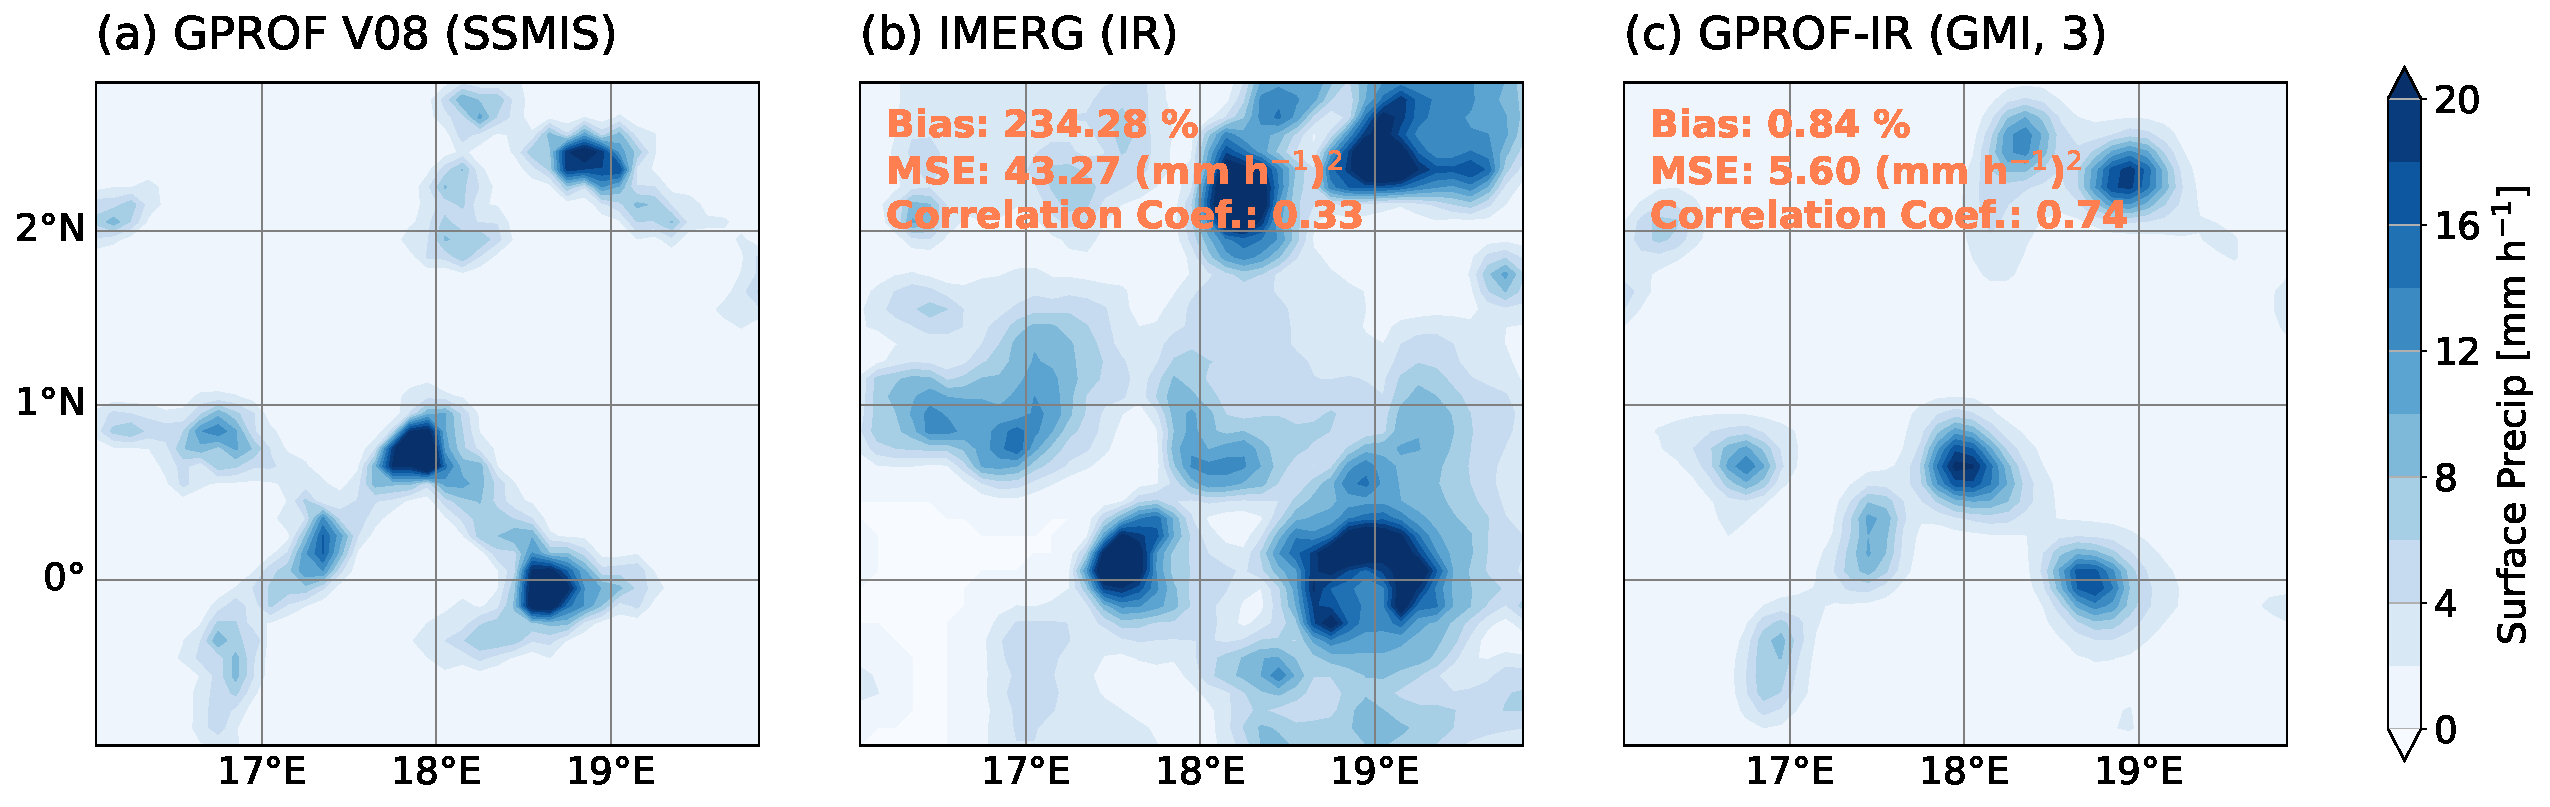
\includegraphics[width=37pc]{figures/figure16.pdf}}
 \caption{
Detailed view of the convective precipitation cells during the SSMIS overpass
occurring at 15:00 UTC shown in Fig. 2. Panel (a) shows the estimates from GPROF
V08, which will be used in IMERG V08; panel (b) shows the IMERG V07 IR
precipitation estimate; panel (c ) shows the corresponding estimates of the
GPROF-IR (GMI, 3) retrieval that will be used to produce precipitation estimates
for IMERG V08
 }\label{fig:evolution_2}
\end{figure}

In addition to being operationally used for IMERG V08, all GPROF-IR retrievals
and their implementation are openly available to the scientific community
\citep{pfreundschuh_gprofir_2026}. Since the retrieval uses only IR observations
as input, it can be easily run using only the CPC gridded IR observations. The
quasi-global availability and high accuracy of the retrieval also provides a
strong baseline for the development of future precipitation retrievals.

\clearpage
%%%%%%%%%%%%%%%%%%%%%%%%%%%%%%%%%%%%%%%%%%%%%%%%%%%%%%%%%%%%%%%%%%%%%
% ACKNOWLEDGMENTS
%%%%%%%%%%%%%%%%%%%%%%%%%%%%%%%%%%%%%%%%%%%%%%%%%%%%%%%%%%%%%%%%%%%%%
\acknowledgments

The work of SP and CDK was supported by NASA grant 80NSSC22K0604.

This study uses modified Copernicus Climate Change Service information. Neither the European Commission nor ECMWF is responsible for any use that may be made of the Copernicus information or data it contains.


\datastatement


The NOAA CPC 4-km gridded IR observations are available from \citet{ncep_cpc_mergir_v1}.

The GPM 2BCMB data are available  from \citet{cmb_data}.

The SatRain dataset is available from \citet{satrain_dataset}.

The OceanRAIN data are available from \citet{ocean_rain_data}.

The ERA5 data are available from \citet{c3s_era5_single_levels}.

The GPCP data are available from \citet{gpcp_v33_precip}.



%%%%%%%%%%%%%%%%%%%%%%%%%%%%%%%%%%%%%%%%%%%%%%%%%%%%%%%%%%%%%%%%%%%%%
% APPENDIXES
%%%%%%%%%%%%%%%%%%%%%%%%%%%%%%%%%%%%%%%%%%%%%%%%%%%%%%%%%%%%%%%%%%%%%

%% If only one appendix, use

%\appendix

%% If more than one appendix, use \appendix[<letter>], e.g.,

%\appendix[A] 

%% Appendix title is necessary! For appendix title:

%\appendixtitle{Title of Appendix}

%%% Appendix section numbering (note, skip \section and begin with \subsection)
%
% \subsection{First primary heading}

% \subsubsection{First secondary heading}

% \paragraph{First tertiary heading}



%%%%%%%%%%%%%%%%%%%%%%%%%%%%%%%%%%%%%%%%%%%%%%%%%%%%%%%%%%%%%%%%%%%%%
% REFERENCES
%%%%%%%%%%%%%%%%%%%%%%%%%%%%%%%%%%%%%%%%%%%%%%%%%%%%%%%%%%%%%%%%%%%%%


\bibliographystyle{ametsocV6}
\bibliography{references}


\end{document}
%%%%%%%%%%%%%%%%%%%%%%%%%%%%%%%%%%%%%%%%%%%%%%%%%%%%%%%%%%%%%%%%%%%%%
% END OF AMSPAPERV6.1.TEX
%%%%%%%%%%%%%%%%%%%%%%%%%%%%%%%%%%%%%%%%%%%%%%%%%%%%%%%%%%%%%%%%%%%%%
